\section{Training Results}\label{sec:results}

We train GP models using the method described in Section \ref{sec:gpmodel}. The training data are evolutioanry tracks in both primary and additional girds as mentioned in Table~\ref{tab:grid}. The role of the additional grid is increasing the grid resolution for evolutionary tracks with the 'hook'. 
%As discussed in the previous section, the kernel function in the 'hook' area are much more complex than other regions , and hence a GP model requires more information to map the feature in this region. 
The total training data includes $\sim$15,000 evolutionary tracks ($\sim$10,000,000 stellar models). Off-grid tracks are split 50-to-50 for validating (in the training progress) and testing (after the training progress) GP models.
The section scenario is applied. For each section, we train a GP model for each output parameter. Each training involves 20,000 training data points and 20,000 validating data points. For the testing dataset, we sample 50, 000 data points in the whole $EEP$ range. Note that we do not use models with $\tau \geq$ 20.0 Gyr, [Fe/H]$_{\rm surf} \leq$ -0.6 dex, or $T_{\rm eff} \geq$ 7000$K$ in testing dataset. 

\subsection{Overview of Results}

We start with training one \textsc{Exact GP} model for the whole $EEP$ range as a standard. Testing errors for this model are listed in Table~\ref{tab:results}. Compared with 2D and 3D cases, testing errors remarkably rise with increasing demission. For example, EI for $T_{\rm eff}$ goes up to 46K, which is much higher than that for the 2D (16K) or the 3D model (24K). 

We then train GP models with the section scenario. We gradually increase the number of sections and track down the changes in testing errors. 
We find that testing EI is not significantly improved when the grid are divided by more than 10 sections. We list the testing errors for different cases in Table~\ref{tab:results}. As it shown that, testing EIs for 10-, 20-, and 100-sections cases are very close. It turns out that the 10-sections case is the most efficient strategy and we take this case as the best result. Following analysis are all based on it. 

A overview of testing errors can also be seen in Figure~\ref{fig:5d_test_vs_input}, where we demonstrate rolling medians and rolling standard deviations of testing errors as a function of input parameters.
%
Median values are approximate along zero in most plots, indicating good agreement between GP predictions and true values.
%
The 68\% confidential intervals are generally small and do not significantly vary. However, the 95\% confidential intervals vary in large dynamic ranges and clearly depend on $M$, $EEP$, and $\rm [Fe/H]_{init}$. The long tails in marginal distributions are similar to what is illustrated in Figure~\ref{fig:2dtest}: GP predictions are relatively poor in some particular regions. Because the systematic uncertainty are not uniform through the parameter space, marginal error distributions do not well describe the systematic uncertainties. We hence investigate systematic uncertainty in a local scale. 

\begin{table*}
	\centering
	\caption{Training and validating errors for GPR Models}
	\label{tab:results}
	\begin{tabular}{cccccccccc}
		\hline
		Model Type&Inputs&$N_{\rm Training}$ &Sampling rate &\multicolumn{5}{c}{Testing Errors (at 68/95/99.7\%)} \\
		 \hline
		 \multicolumn{4}{c}{}& $T_{\rm eff}$ &$\log g$  &$R$  &[Fe/H]$_{\rm surf}$   &$\tau$ \\
		 \multicolumn{4}{c}{}&  (K)& ($10^{-3}$dex) & ($10^{-3}R_{\odot}$)  &  ($10^{-3}$dex)  & ($10^{-2}$Gyr) \\		 
		 \hline
		 Exact GP & 2D & 20,000 x 1 &96\% & 1/5/11 & 1/3/8 & 2/6/14 & 0.5/2/12 &  1/3/9 \\
		 %SVGP & 2D & 2,000 x 10  &96\% & 1/5/11 & 1/4/10 & 3/7/14  & 0.3/2/14 & 1/4/10  \\
		 \hline		 
		 Exact GP & 3D & 20,000 x 1 & 5\% & 2/6/16 & 1/4/10 & 3/7/17 &  2/6/22 & 2/7/22 \\
		 %Exact GP (5 sections) & 3D & 20,000 x 5 & 20\% & 2/6/17 &1/4/10 & 3/7/16& 1/3/18& 2/6/19\\
		  Exact GP (10 sections) & 3D & 20,000 x 10 & 50\% & 2/5/15 &1/4/11 & 2/7/17& 1/3/20& 2/6/19\\
		% SVGP (too slow) & 3D & 2,000 x 50 & 25\% & 3/7/16 & \\
		 %SVGP (too slow)  & 3D & 5,000 x 20 & 25\% & 2/7/15 & & & & & \\
		 %GIGP (Relu + normal data)& 3D & 100K & 25\% & 2/7/14  & & & & & \\
		 %GIGP (Relu + normal data)& 3D & 200K & 50\% & 4/8/17  & & & & & \\
		 %GIGP (Relu + grid data)& 3D & 220K & 50\% & 5/10/28 & & & & & \\
		 %GIGP (elu + grid data)& 3D & 220K & 50\% & 7/12/29 & & & & & \\
		 %\hline
		 %Exact GP (multitask) & 3D & 20,000 x 1 & 5\% & memory  &  &  &   &  \\
		  \hline		 
		 Exact GP & 5D & 20,000 x 1 & 0.2\% & 3/9/34 & 2/5/18 & 4/11/36 & 2/7/30 & 3/9/27  \\
		 Exact GP (3 sections) & 5D& 20,000 x 3 & 0.6\% &  3/8/27 & 2/5/18 & 3/7/26 & 1/4/24 &3/7/22 \\
		 %Exact GP (3 sections) & 5D& 20,000 x 3 & 0.6\% &  2.5/7.7/27.4 & 15/45/177 & 26/73/257 & 9/42/236 &26/73/226 \\
		 Exact GP (5 sections) & 5D& 20,000 x 5 & 1\% &  2/7/25 & 1/4/15 & 3/7/24 & 1/4/21 &2/6/22 \\
		 %Exact GP (5 sections) & 5D& 20,000 x 5 & 1\% &  2.4/7.2/24.8 & 13/39/152 & 25/71/242 & 9/39/207 &21/64/215 \\
		 Exact GP (10 sections) & 5D& 20,000 x 10 & 2\% & 2/7/27  & 1/4/14 & 2/7/26 &1/4/20 & 2/6/21\\
		 %Exact GP (10 sections) & 5D& 20,000 x 10 & 2\% & 2.4/7.1/26.8  & 14/40/141 & 24/70/263 &9/37/196 & 21/64/208\\
		 Exact GP (20 sections) & 5D& 20,000 x 20 & 4\% & 2/7/26  & 1/4/14 & 2/7/27 &1/3/18 & 2/6/22 \\
		 %Exact GP (20 sections) & 5D& 20,000 x 20 & 4\% & 2.2/6.9/26.1  & 13/38/141 & 24/72/290 &9/32/182 & 19/61/218 \\
		  Exact GP (100 sections) & 5D& 20,000 x 100 & 20\% & 2/7/25  & 1/4/14 & 2/7/26 &1/3/17 & 2/6/18 \\
		 % Exact GP (100 sections) & 5D& 20,000 x 100 & 20\% & 2.2/6.7/25.8  & 13/36/157 & 23/67/283 &8/34/185 & 19/59/190\\
		 %GIGP (Elu) & 5D & 10 x10,000 & 1\% & 5/12/34 & & & & \\
		 %GIGP (Relu) & 5D & 10 x10,000 & 1\% & 6/13/47 & & & & \\
		 %GIGP & 5D &  & 2\%, 5\%, 10\%, 25\%  & memory & & & & \\
		% \hline
		 % \multicolumn{9}{c}{GP a subset of 5D data-hook}\\
		 %\hline
		 %Exact GP EEP = 0.2-0.4 & 5D & 20,000 x 1 & 1\% & 2/7/20 &&&\\
		 %Exact GP EEP = 0.3-0.4 & 5D & 20,000 x 1 & 2\% & 3/8/21  &&&\\
		 %Exact GP EEP = 0.3-0.35 & 5D & 20,000 x 1 & 3\% & 2/7/17 &&&\\
		  %Exact GP EEP = 0.3-0.32 & 5D & 20,000 x 1 & 8\% & 2/5/14 &&&\\
		 %Exact GP EEP = 0.3-0.31 & 5D & 20,000 x 1 & 16\% & 2/4/13  &&&\\
		  \hline
	\end{tabular}
\end{table*}

\begin{figure*}
	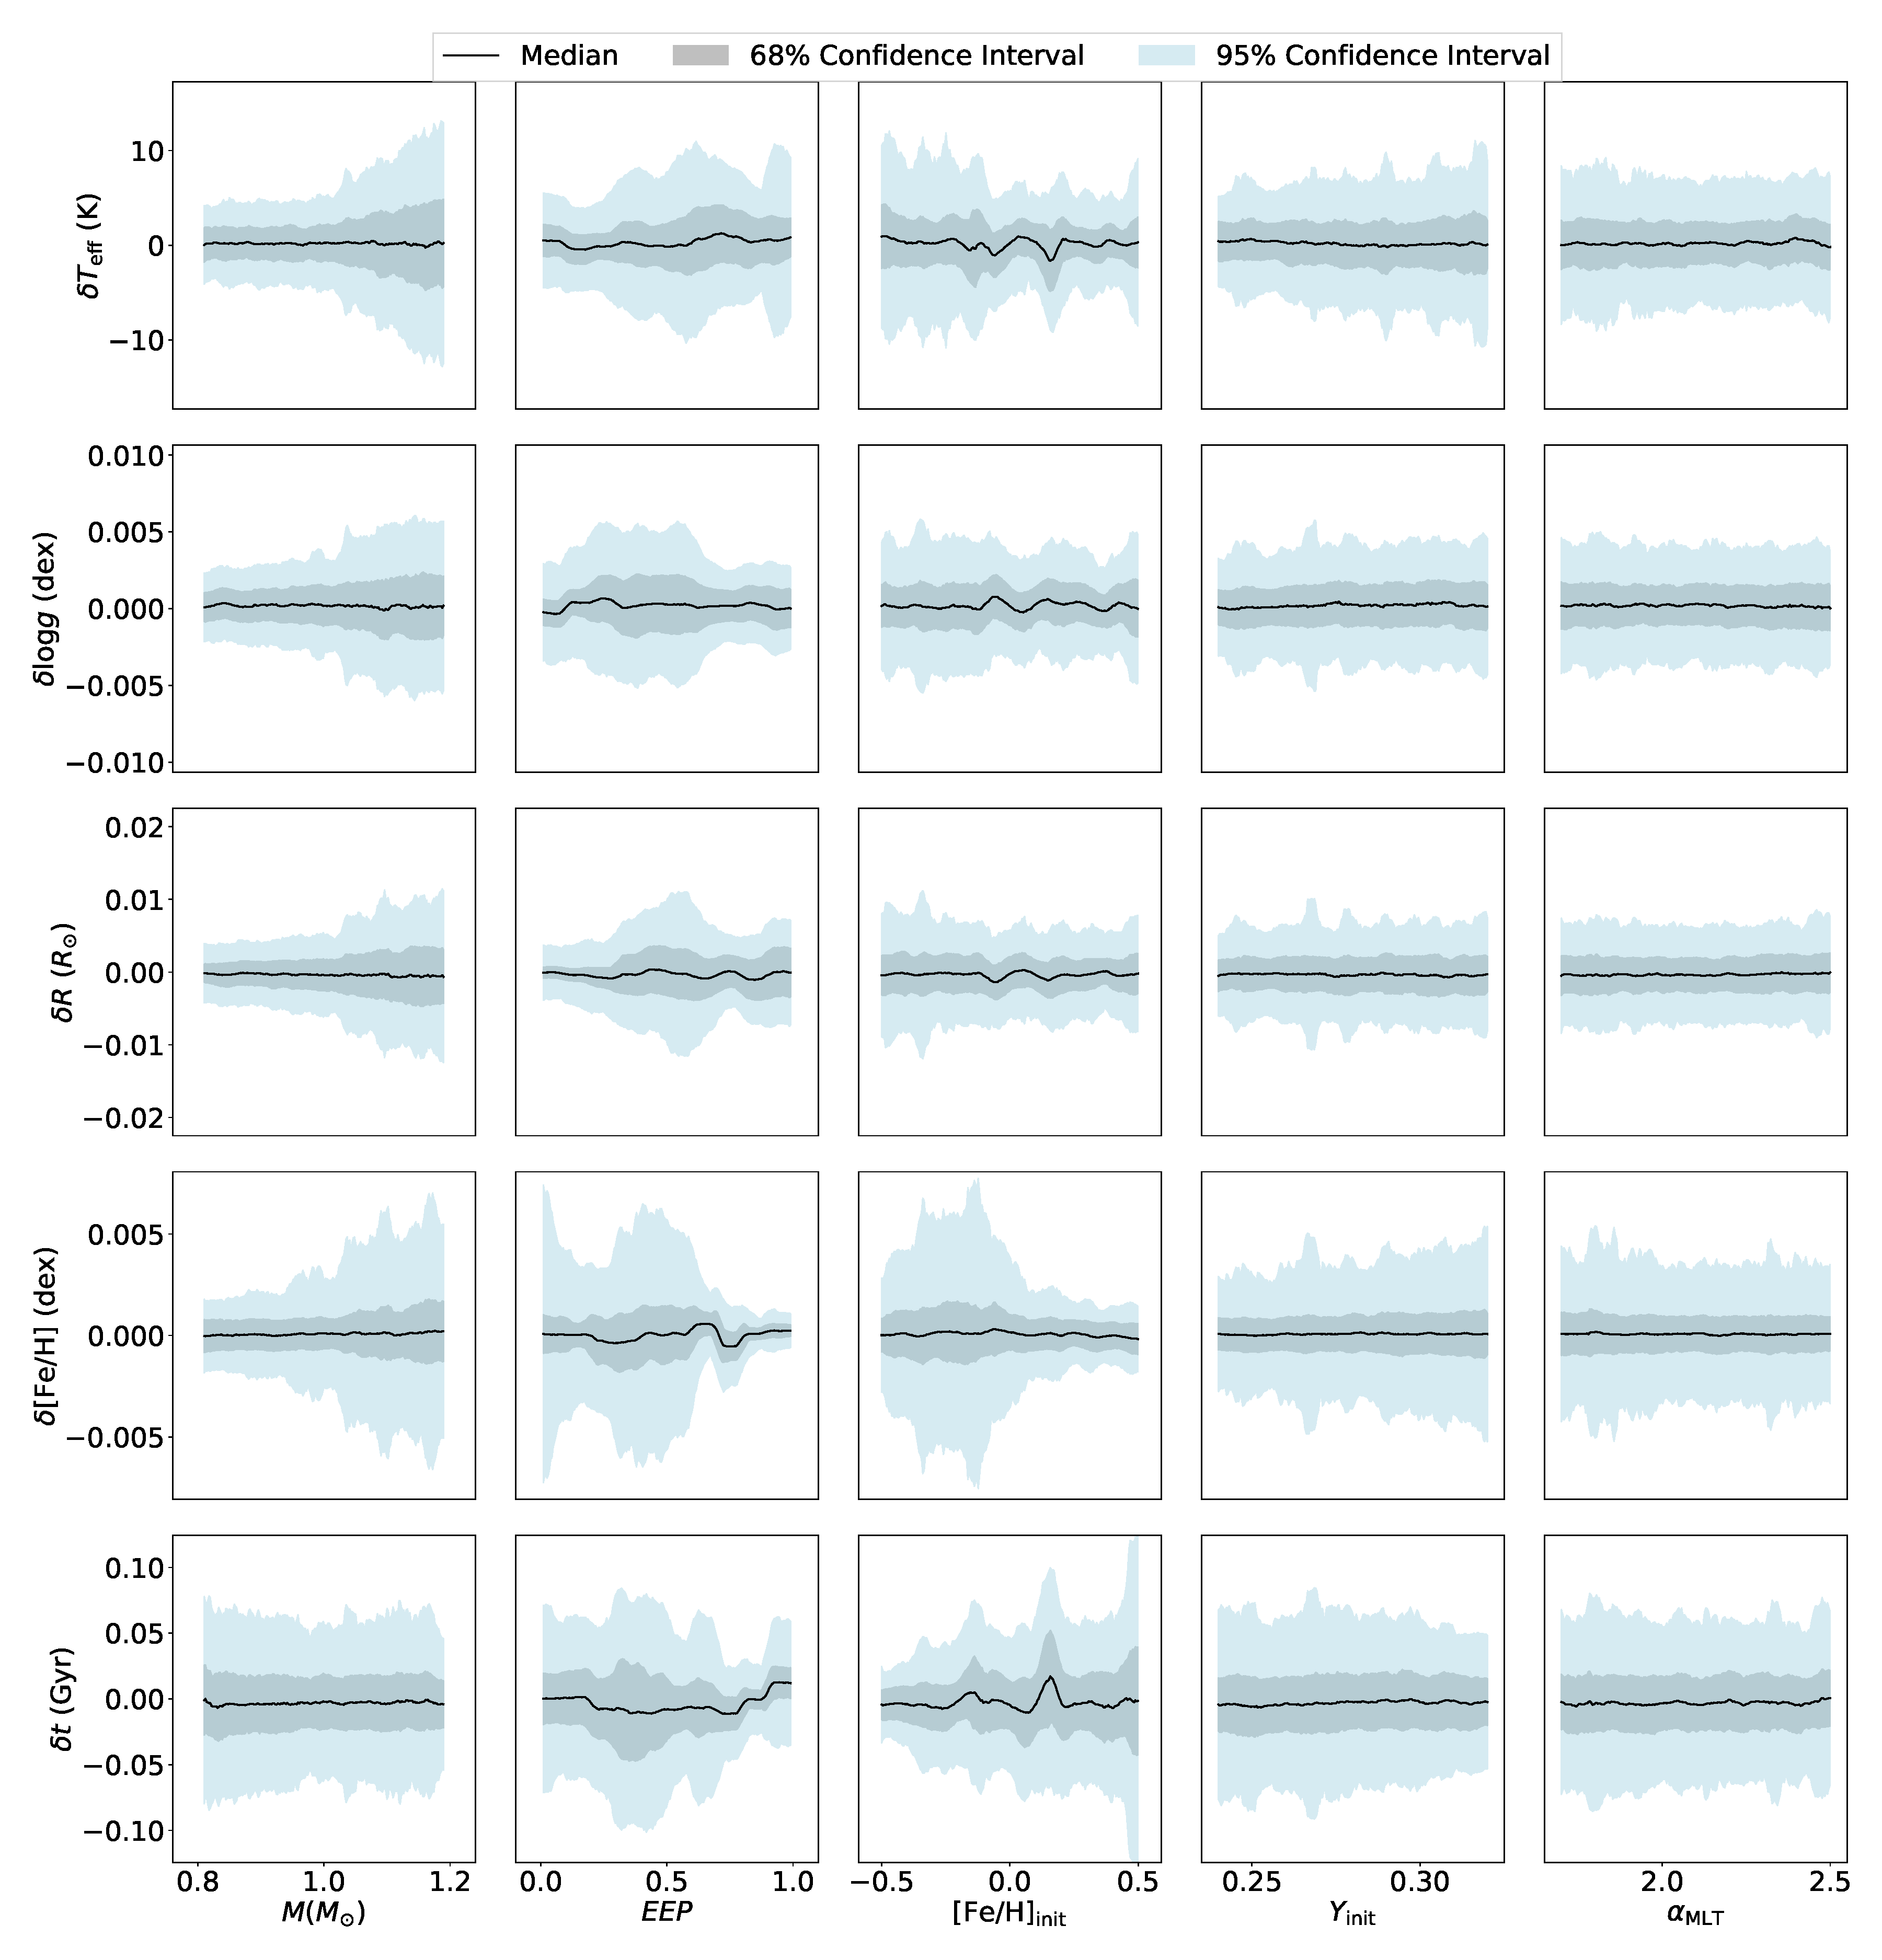
\includegraphics[width=2.0\columnwidth]{ 5d-testing_vs_inputs.pdf}
    \caption{ Roll medians and 68/95\% confidential intervals of testing errors against GP model  inputs. Black solid lines indicate the median value; grey and blue shadowes represent the 68\% and 95\% confidential interval. Testing errors of $T_{\rm eff}$, $\log g$, and $R$ mainly depend on $M$ and $EEP$. Metallicity error strongly depends on $M$, $EEP$, and [Fe/H]$_{\rm init}$, and age error has a significant correlation to $EEP$ and [Fe/H]$_{\rm init}$. However, testing errors do not obviously relate to $Y_{\rm init}$ or $\alpha_{\rm MLT}$. } 
  \label{fig:5d_test_vs_input}
\end{figure*}
%

\subsection{Mapping Systematical Uncertainties using another GP model}\label{sec:sys}

As shown in Figure~\ref{fig:5d_test_vs_input}, systematical uncertainties relate to $M$, $EEP$, and [Fe/H]$_{\rm init}$ but not to $Y_{\rm init}$ or $\alpha_{\rm MLT}$.  Thus, a comprehensive model for the systematical uncertainty can be described as a function of $M$, $EEP$, and [Fe/H]$_{\rm init}$. In the $M$-$EEP$-$\rm [Fe/H]_{init}$ space, we divide this 3D space into equal-size segments and examine local error distributions. 
The choice of segment size matters. It needs to be small enough for only presenting the local feature, but it can not be very small so that there are not enough data points for proper statistical analysis. 
%
To find an appropriate size, we apply a statistic test. The purpose of the test is to check wether the local distribution has a tail feature. The condition we apply is either the ratio between 68\% and 95\% confidential intervals less than 2.5, or the ratio between 68\% and 99.7\% confidential intervals less than 4. 
%
After several attempts, we decide to divide the input range into 40 equally spaced segments for $M$, 50 for $EEP$, and 20 for [Fe/H]$_{\rm init}$. Hence there are 43,911 (41 x 21 x 51) gird points. We compute a rolling standard deviation for each grid point by using the data in a 3-segments (1.5 previous and 1.5 after) range across each demission. The statistic test shows that $\sim 90\%$ points meeting the above condition. 

We present local systematic uncertainties for $T_{\rm eff}$ ($\sigma T_{\rm eff}$) on the $M-EEP$ diagram in Figure \ref{fig:5d_sys_teff}. As it can be seen that, local $\sigma T_{\rm eff}$ values are mostly below $\sim$4K in the low-mass regions and raise up when mass is greater than 1.05$\rm M_{\odot}$. More important, there are substructures randomly appear in the parameter space. 
We visually inspect local systematic uncertainties for all output parameters and find similar features. 
%The substructures are expected because this is the residual of a flexible kernel function. 
Because of the existence of substructures, it is not convinced to describe the systematic uncertainty with any simple mathematical expressions. We hence use another GP model (GP-SYS model here after) to map three fundamental inputs ($M$, $EEP$, and [Fe/H]$_{\rm init}$) to local systematic uncertainty of each output parameter.   

Here we discuss how we set up the GP-SYS model. 
There are 43,911 data points in total. We randomly select 32,000 data points as the training dataset and use the rest 11,311 data points as the validating dataset. Because the training data size exceeds the 20,000 limit for \textsc{Exact GP}, we use other approach for the large data sample.
%
As discussed in Section \ref{sec:gpmodel}, the SVGP framework can be applied for when the kernel function is not very complex. It hence suitable for training the systematic uncertainty. We use 10,000 inducing points which are randomly selected in the 3D space. The training data is split into 10 batches for the SVGP training. 
%
We use a constant mean function and the RBF kernel because the data distribution is smooth. The variational evidence lower bound (ELBO) is adopted as the loss function. This approach is designed for when there is too much data for the exact inference. We set up Early Stopping by tracking the RMSE value of validating data. The training progress terminates when the RMSE value stops decreasing for 30 iterations.
The likelihood function and the optimiser are same as those for training GP-Grid models. 
Our set up for the GP-SYS model is listed as follow.
\begin{itemize}
\item Model Type: SVGP with 10,000 inducing number. 
\item Model Inputs: $M$, $EEP$, and [Fe/H]$_{\rm init}$
\item Model Outputs: $\sigma_{T_{\rm eff}}$, $\sigma_{\log g}$, $\sigma_{R}$, $\sigma_{\rm [Fe/H]_{surf}}$, and $\sigma_{\tau}$.
\item Training dataset: 3200 x 10 data points
\item Validating dataset: 11,311 data points
\item Kernel: RBF (for all outputs)
\item Mean Function: Constant Mean Function 
\item Likelihood Function: Gaussian Likelihood Function
\item Loss Function: The variational evidence lower bound (ELBO) 
\item Optimiser: Adam including AMSGRAD variant
\item Early Stoping: when validating RMSE stops decreasing for 30 iterations
\end{itemize}    


\begin{figure}
	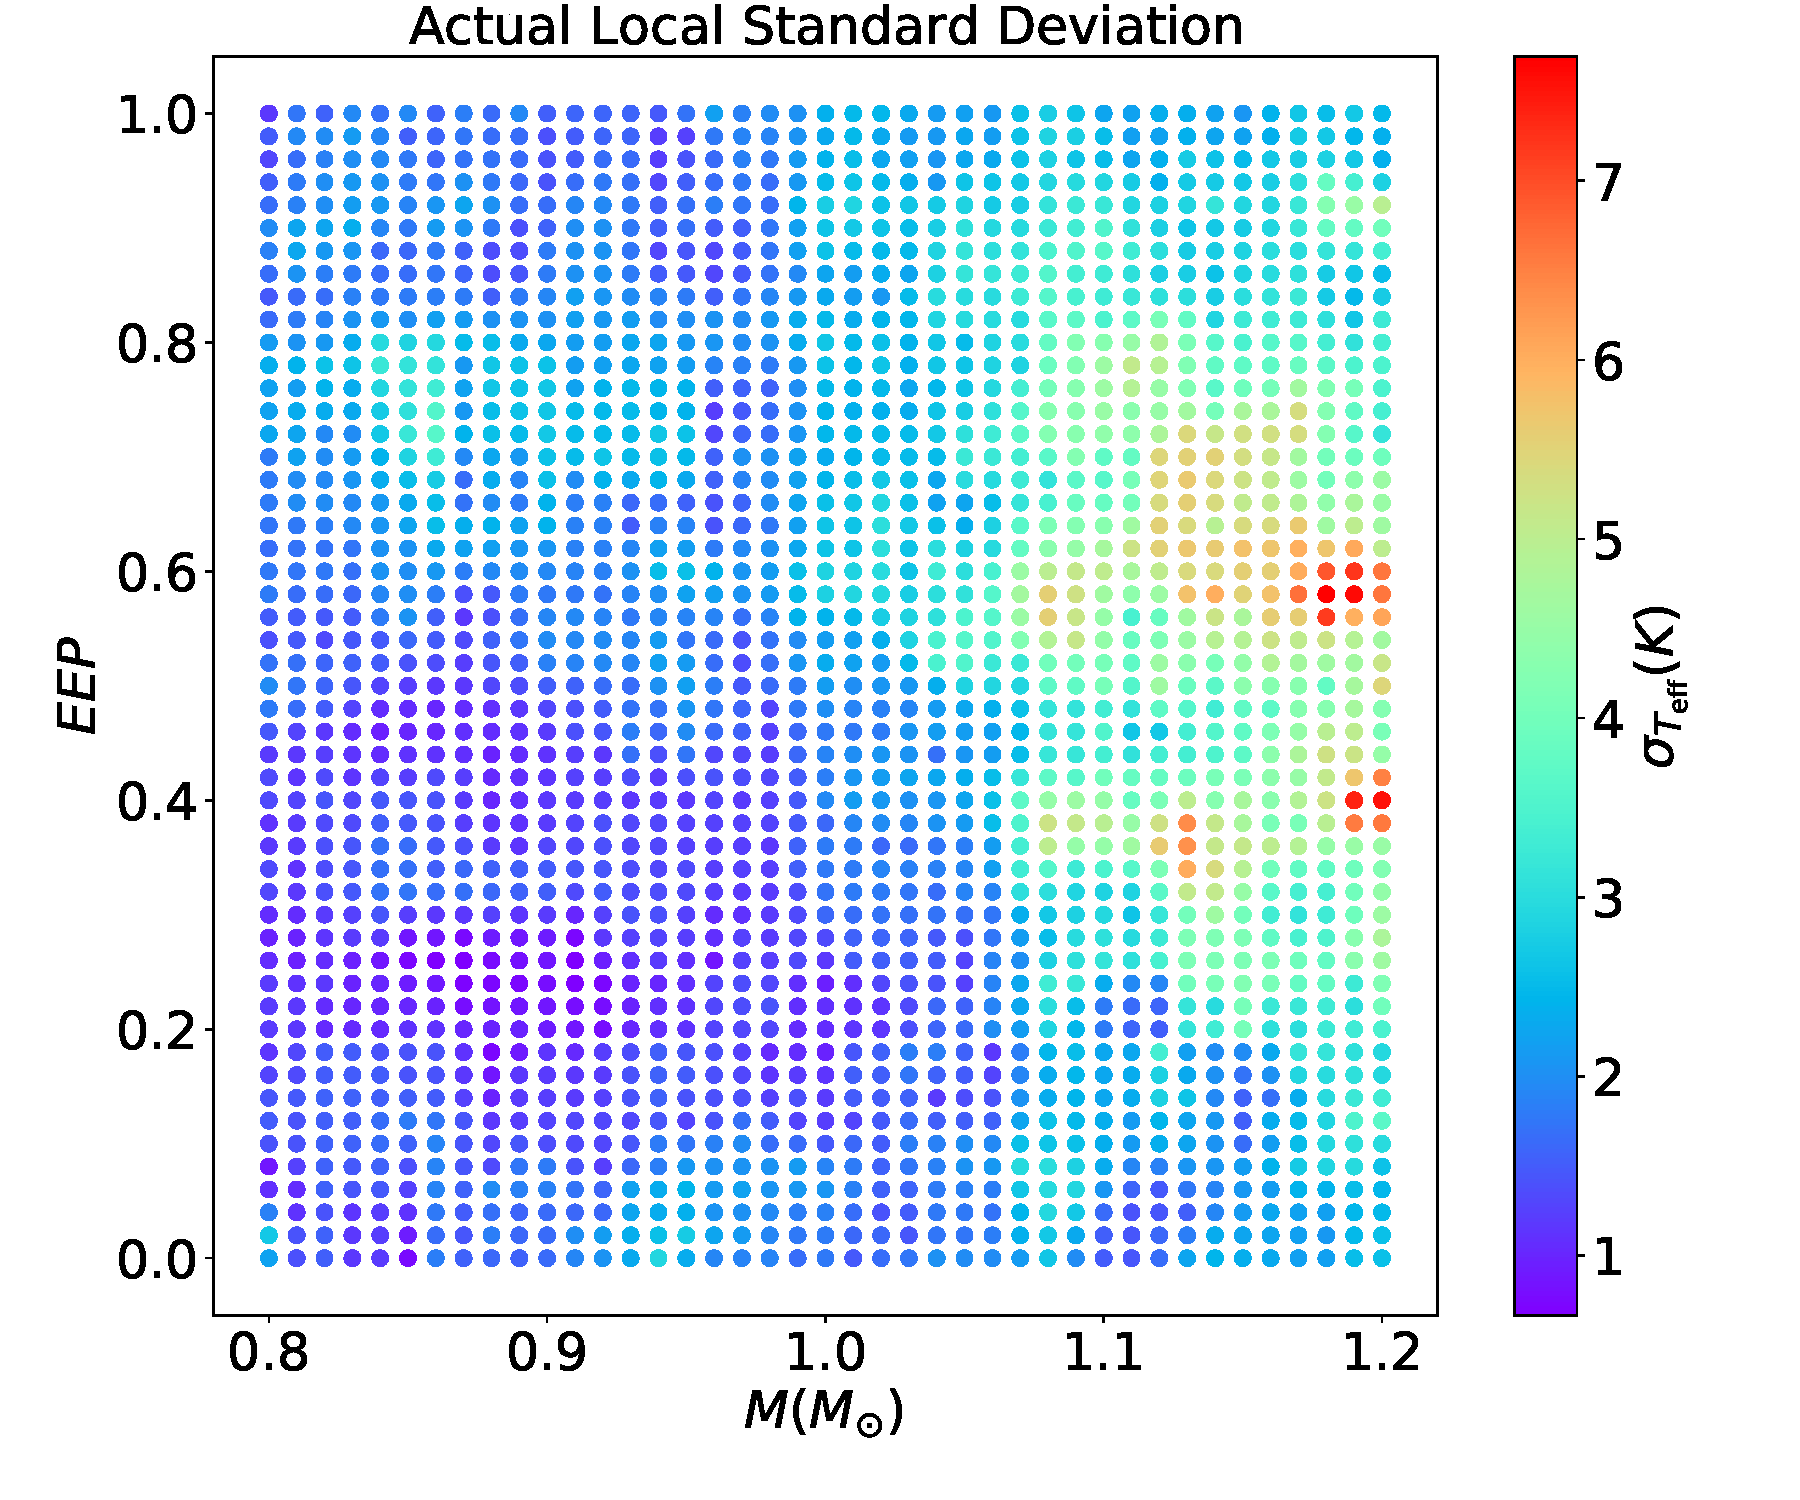
\includegraphics[width=1.0\columnwidth]{5d_sys_teff.pdf}
	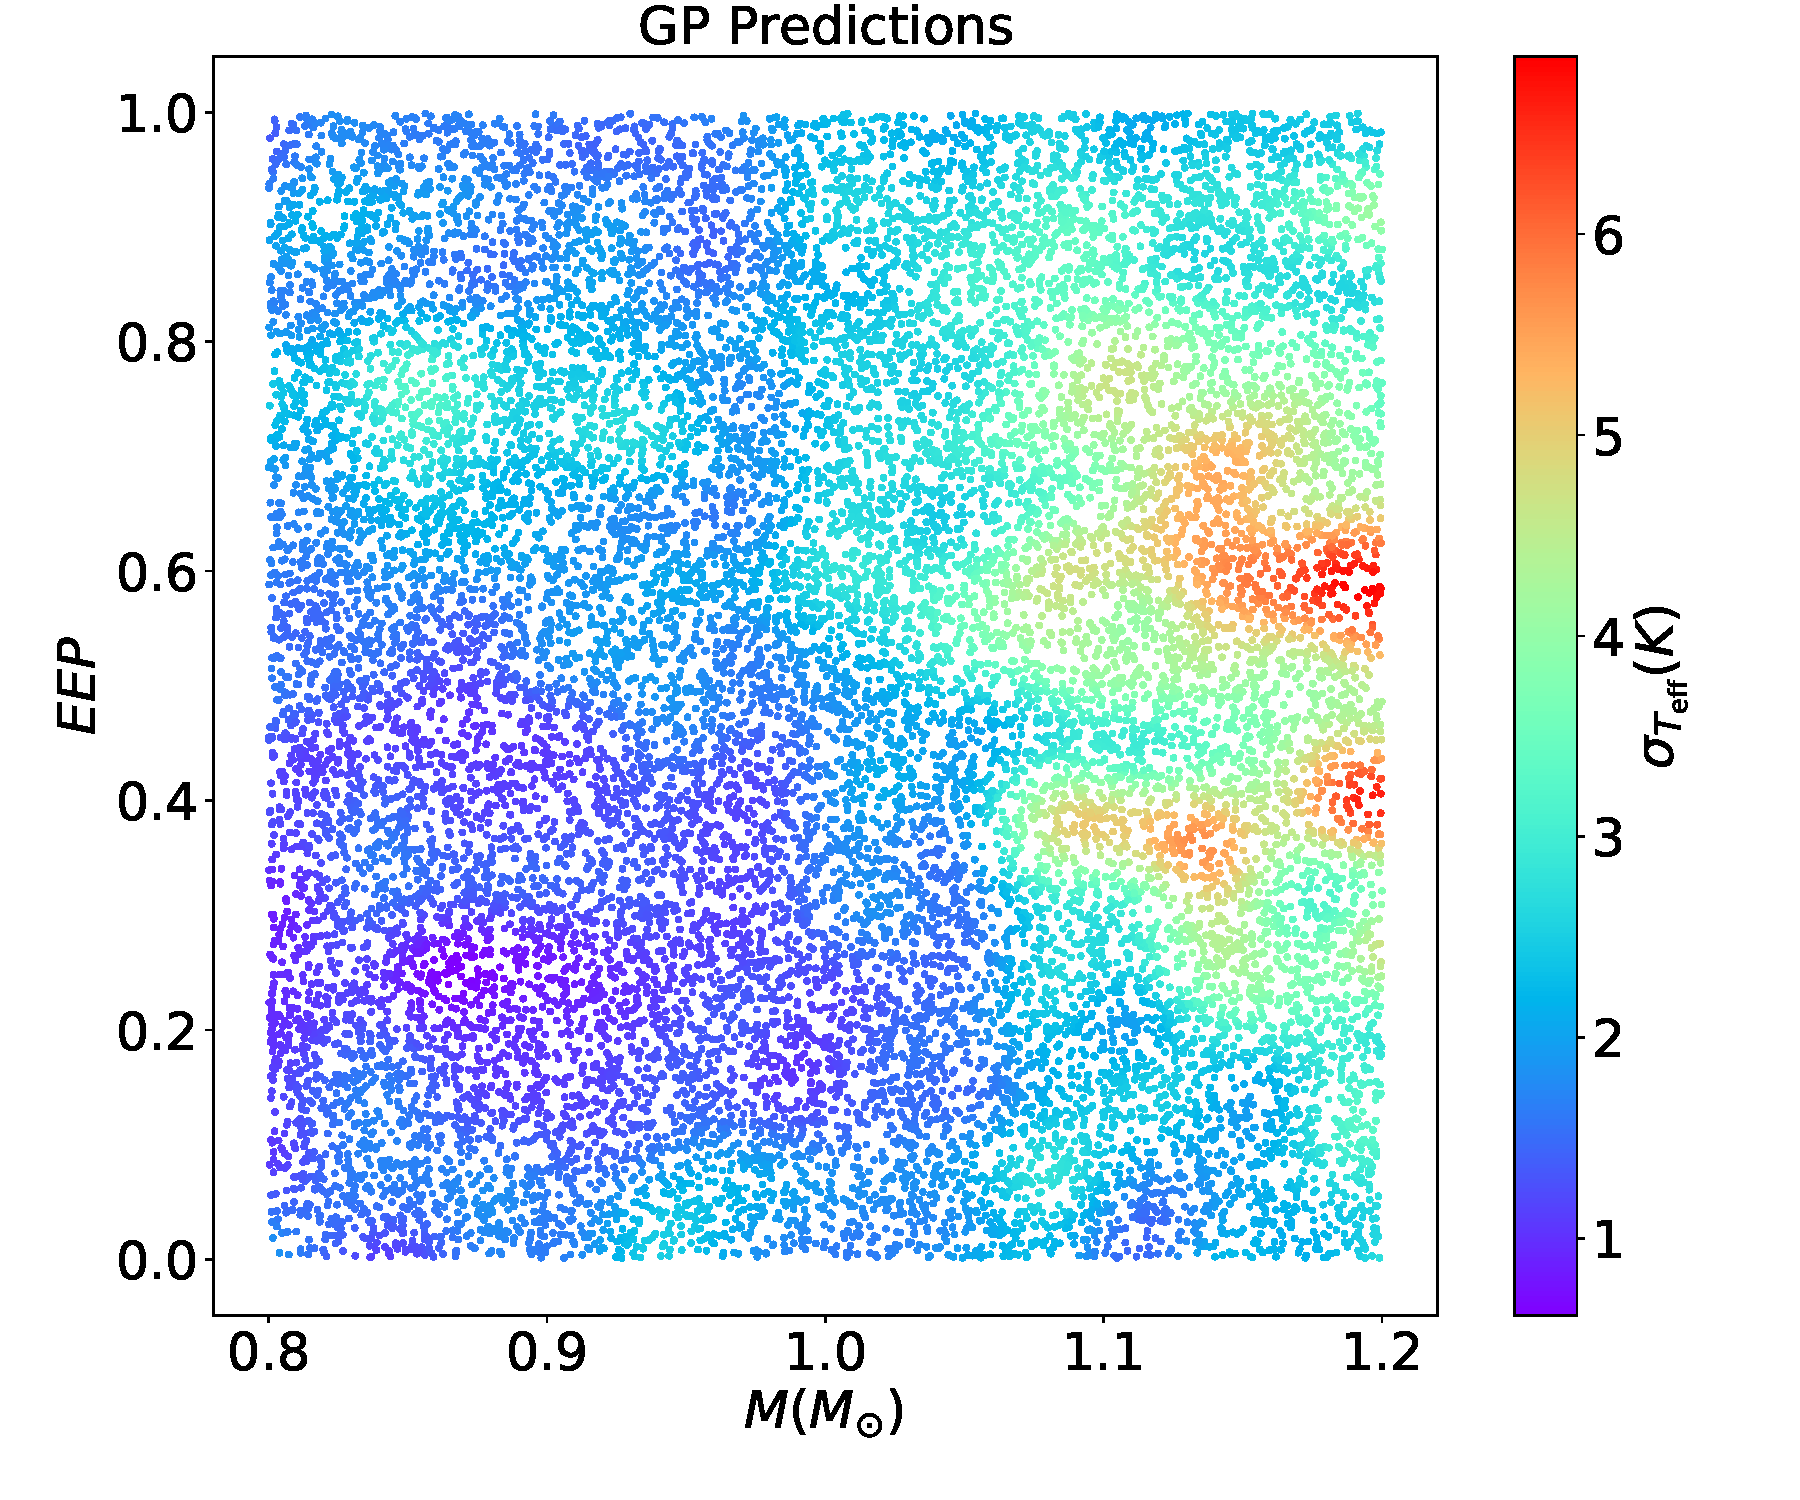
\includegraphics[width=1.0\columnwidth]{5d_sys_effective_T_std_predictions.pdf}
    \caption{Local systematic uncertainty (1-$\sigma$) for $T_{\rm eff}$ on the $M - EEP$ diagram for [Fe/H]$_{\rm init}$ = 0.0. The actual distribution is on the top and GP predictions are presented at the bottom.} 
  \label{fig:5d_sys_teff}
\end{figure}

We train GP-SYS models with the above method. Final models show good agreement with validating data. For instance, the average validating error for $\sigma_{T_{\rm eff}}$ is only 0.15K. For other output parameters, we summary the results in Table \ref{tab:sys}.
%
Figure \ref{fig:5d_sys_teff} includes a comparison between the actual and the GP-trained $\sigma_{T_{\rm eff}}$. It shows that the GP-SYS model well reproduces the $\sigma_{T_{\rm eff}}$ distributions. 

\begin{table}
	\centering
	\caption{Residual of GP models for systematic uncertainty}
	\label{tab:sys}
	\begin{tabular}{lc}
		\hline
		GP output& Average Validating Errors (ABS) \\
		\hline
		$\sigma_{T_{\rm eff}}$  (K) & 0.15 \\
		$\sigma_{\log g}$  ($10^{-3}$dex)   & 0.08 \\
		$\sigma_{R}$ ($10^{-3}R_{\odot}$)   & 0.2 \\
		$\sigma_{\rm [Fe/H]_{\rm surf}}$ ($10^{-3}$dex) & 0.09 \\
		$\sigma_{\tau}$ ($10^{-2}$ Gyr)  & 0.2\\
		%$\sigma_{\Delta\nu} (\mu Hz)$ & 0.01\\
		  \hline
	\end{tabular}
\end{table}


\section{Augmenting the MESA Grid}\label{sec:augmentation}

\subsection{A GP-Trained Model Set}

Now we have GP-Grid models for predicting observable outputs and GP-SYS models for estimate their local systematical uncertainties. 
In Figure~\ref{fig:5d_augmentation}, we demonstrate a GP-trained Kiel diagram comparing with the stellar grid. It shows that GP has transformed the sparse model grid into a non-sparse model set. 
%
Here we generate a GP-Trained model set to augment the stellar grid. We randomly sample 5,000,000 model data points with a flat distribution on each input demission. We then predict observable outputs with GP-Grid models and systematic uncertainties with GP-SYS models. 
%
This GP-trained model set hence includes five fundamental inputs ($M$, $EEP$, [Fe/H]$_{\rm init}$, $Y_{\rm init}$, and $\alpha_{\rm MLT}$), five outputs, ($T_{\rm eff}$, $\log g$,  $R$,  [Fe/H]$_{\rm surf}$, and  $\tau$), and five systematic uncertainties ($\sigma_{T_{\rm eff}}$, $\sigma_{\log g}$,  $\sigma_{R}$,  $\sigma_{\rm [Fe/H]_{\rm surf}}$, and $\sigma_{\tau}$). This model set can be downloaded at \url{a-place-for-data}. 

\begin{figure*}
	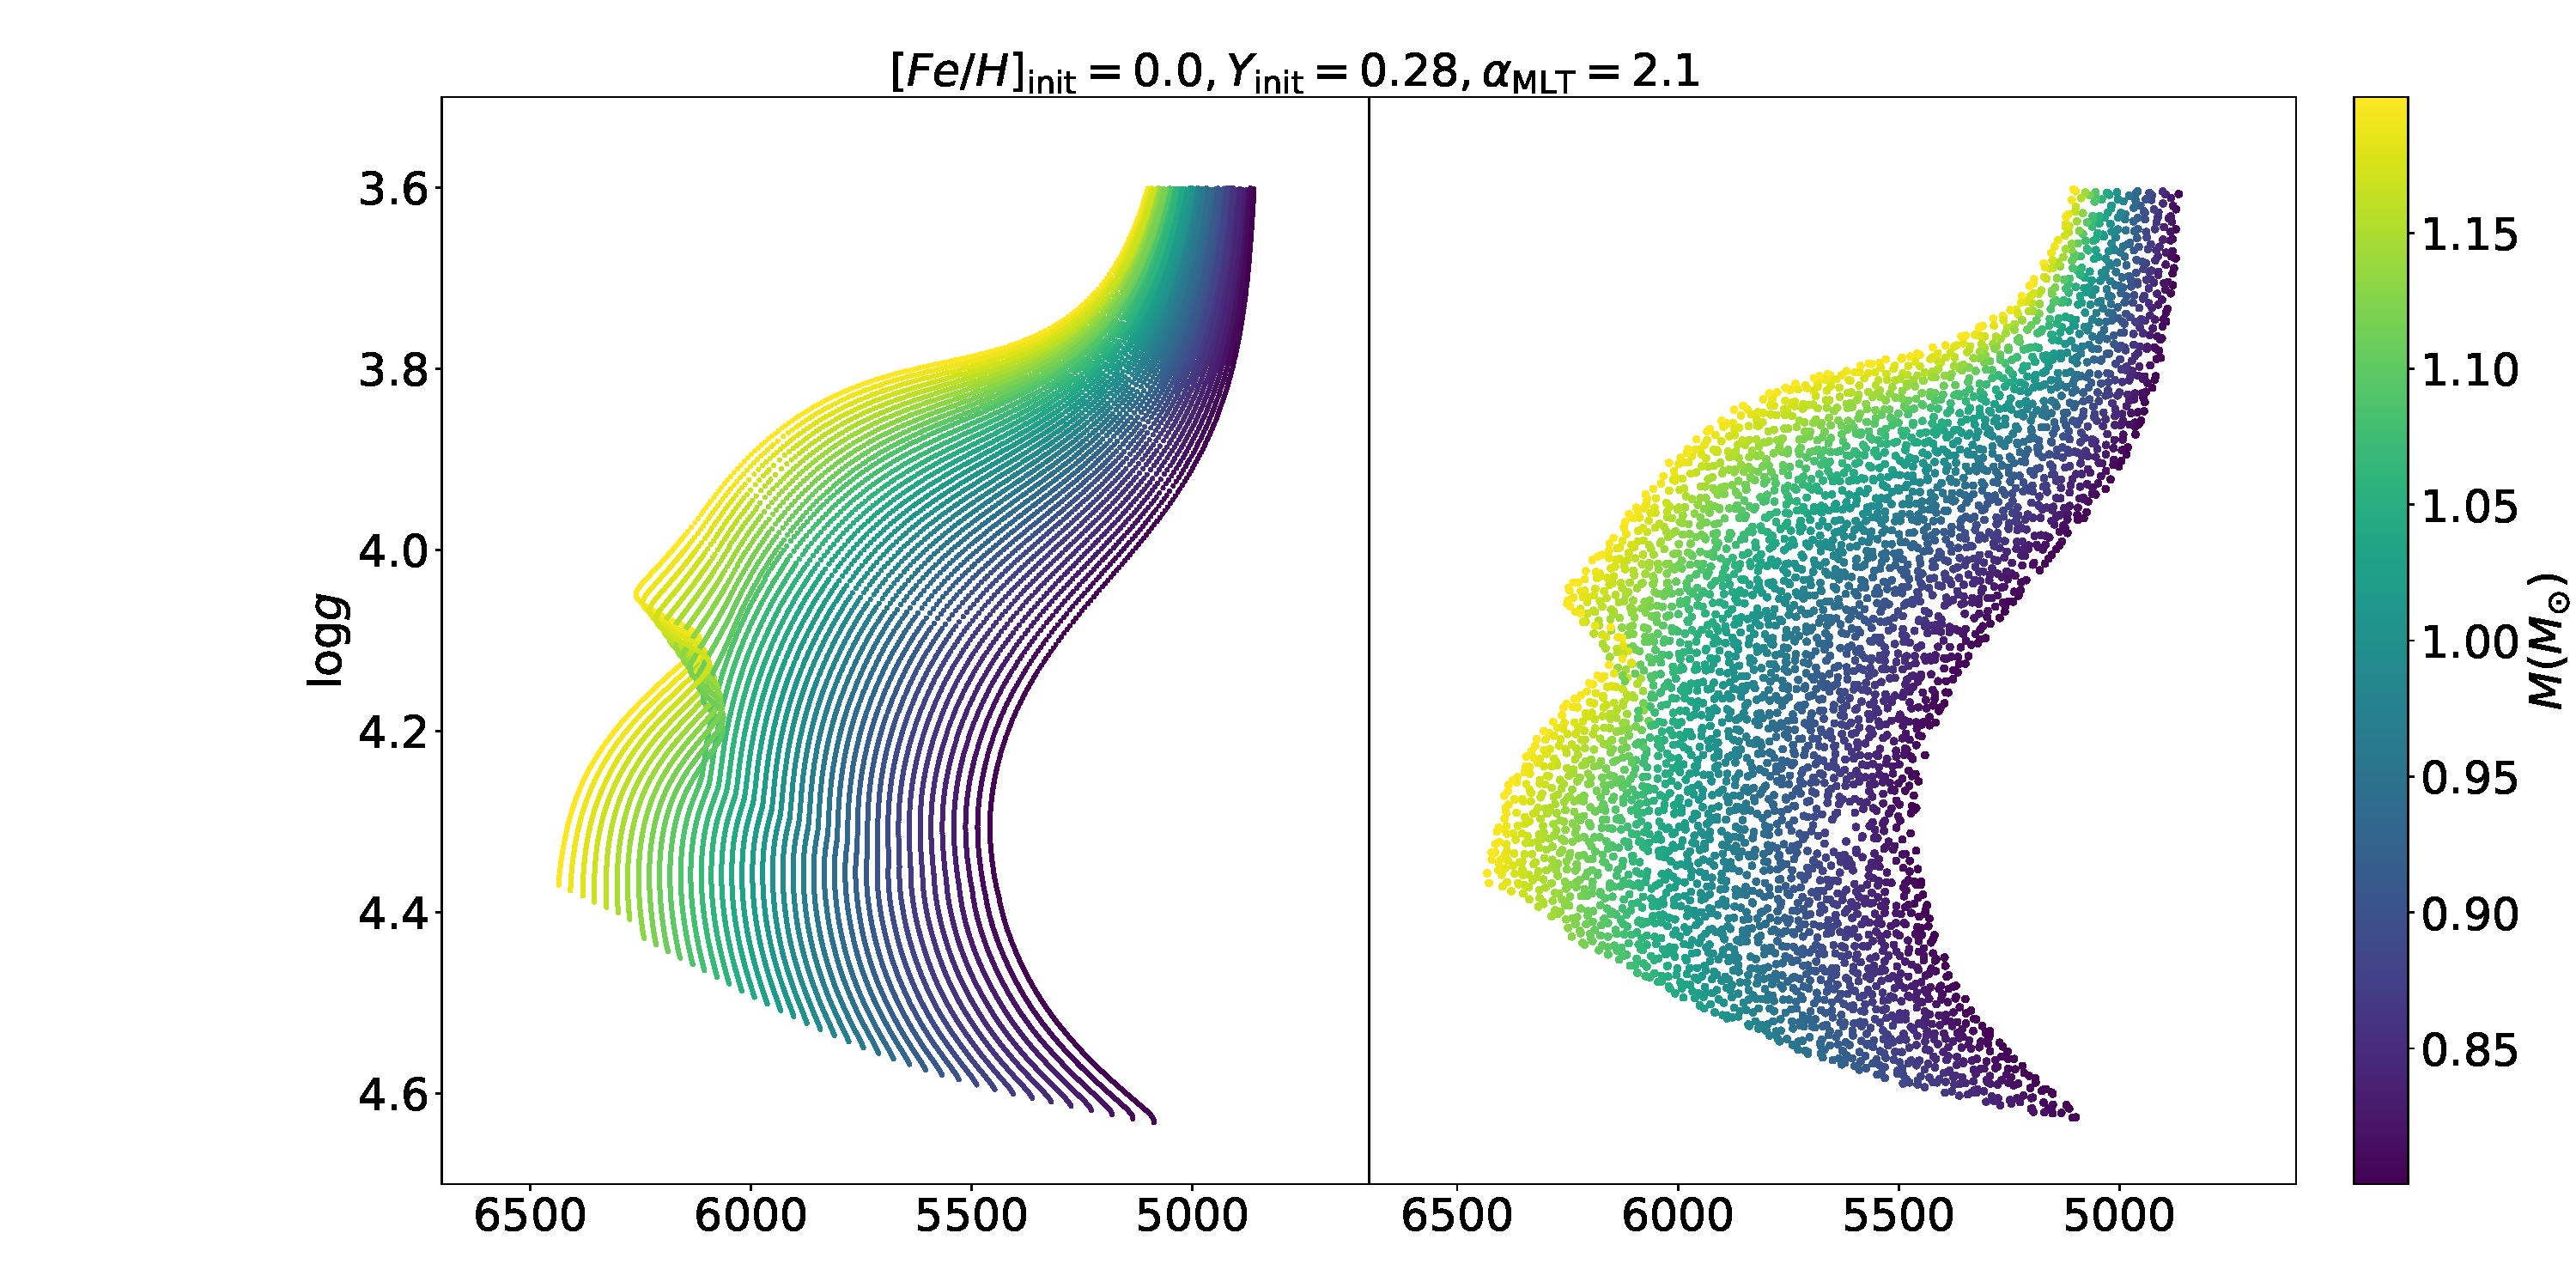
\includegraphics[width=1.3\columnwidth]{5d-au-mass.pdf}
	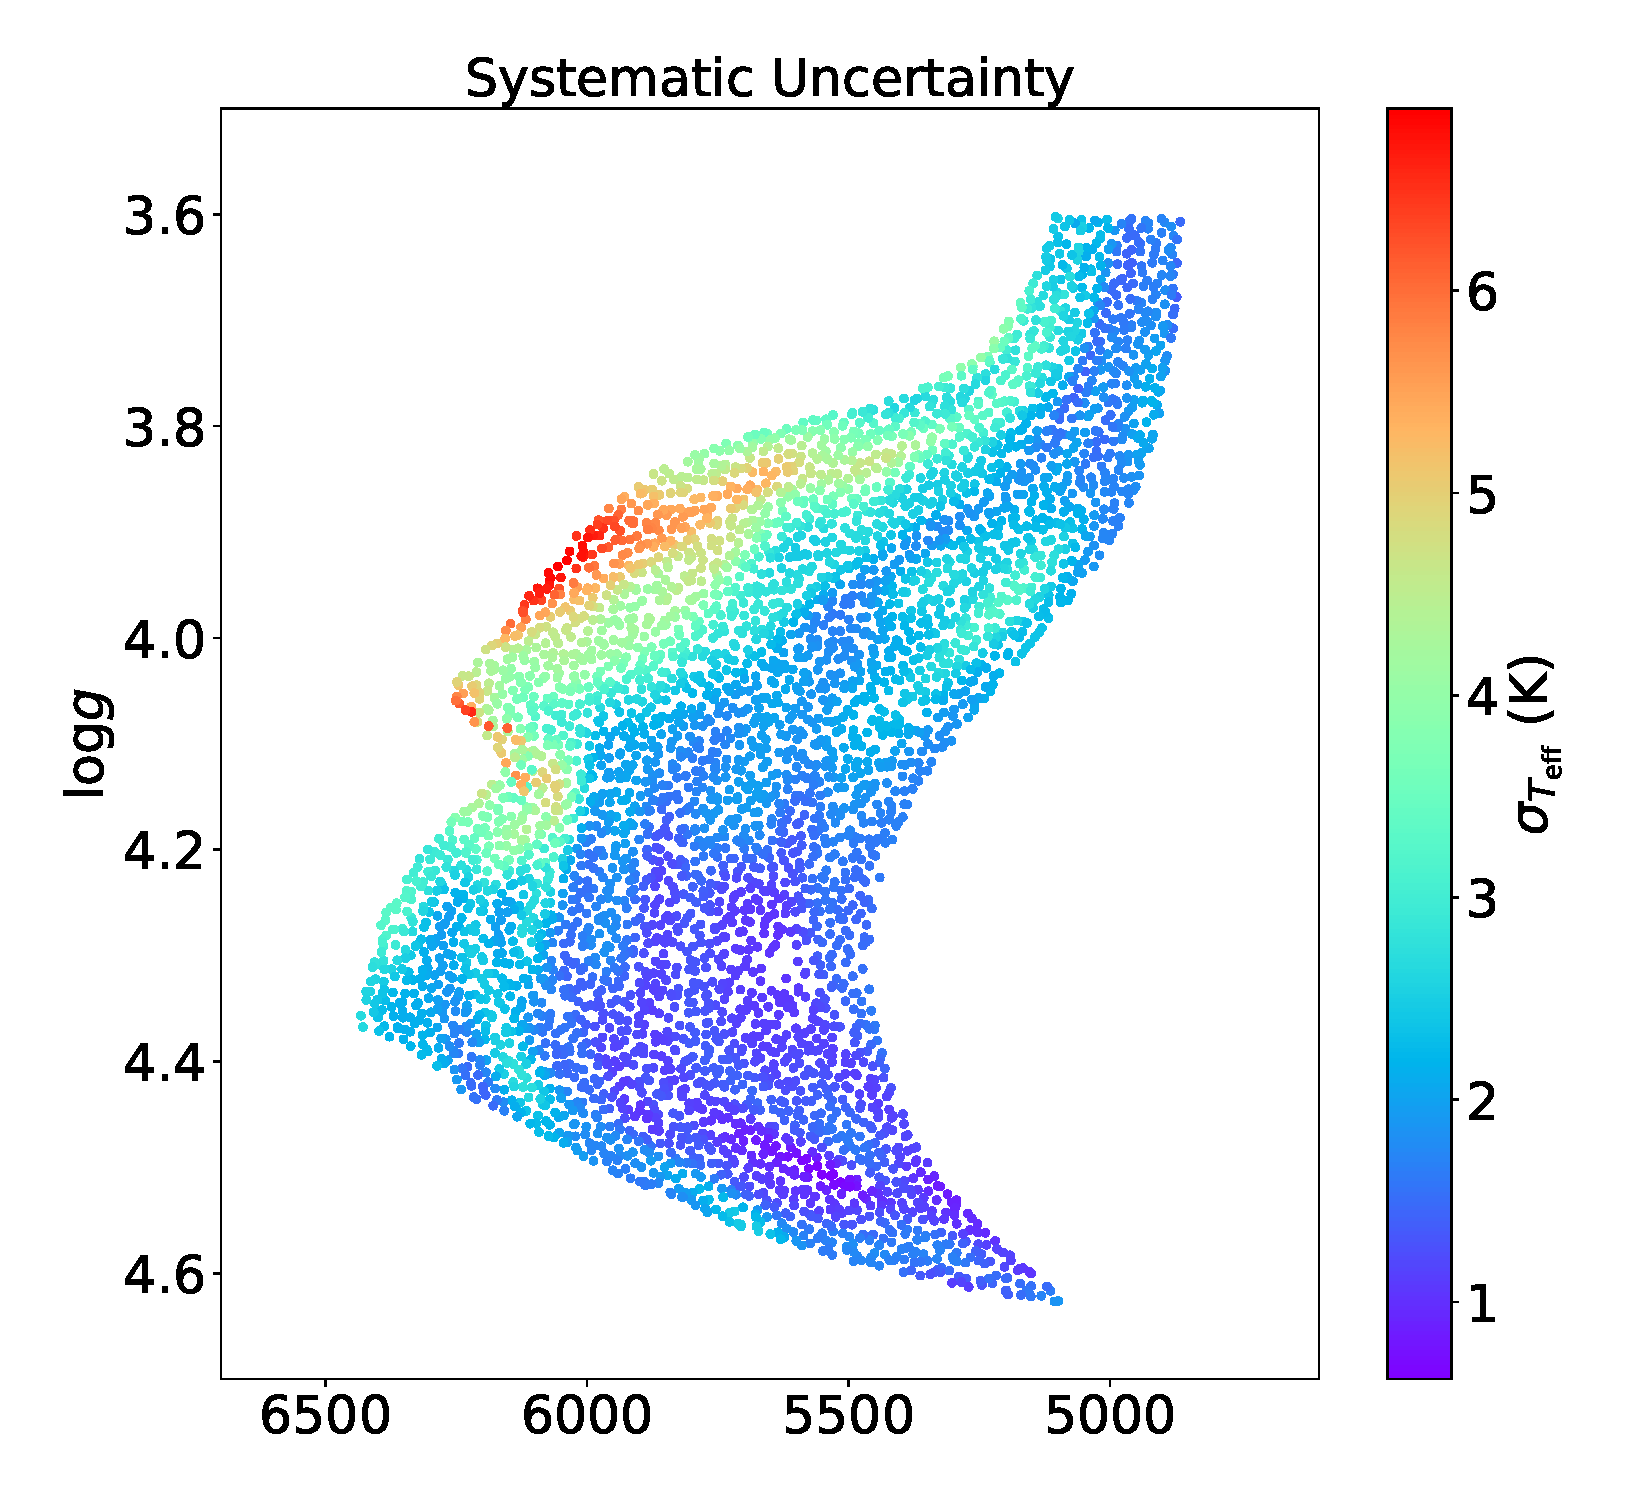
\includegraphics[width=0.7\columnwidth]{5d-au-mass-sys.pdf}
	%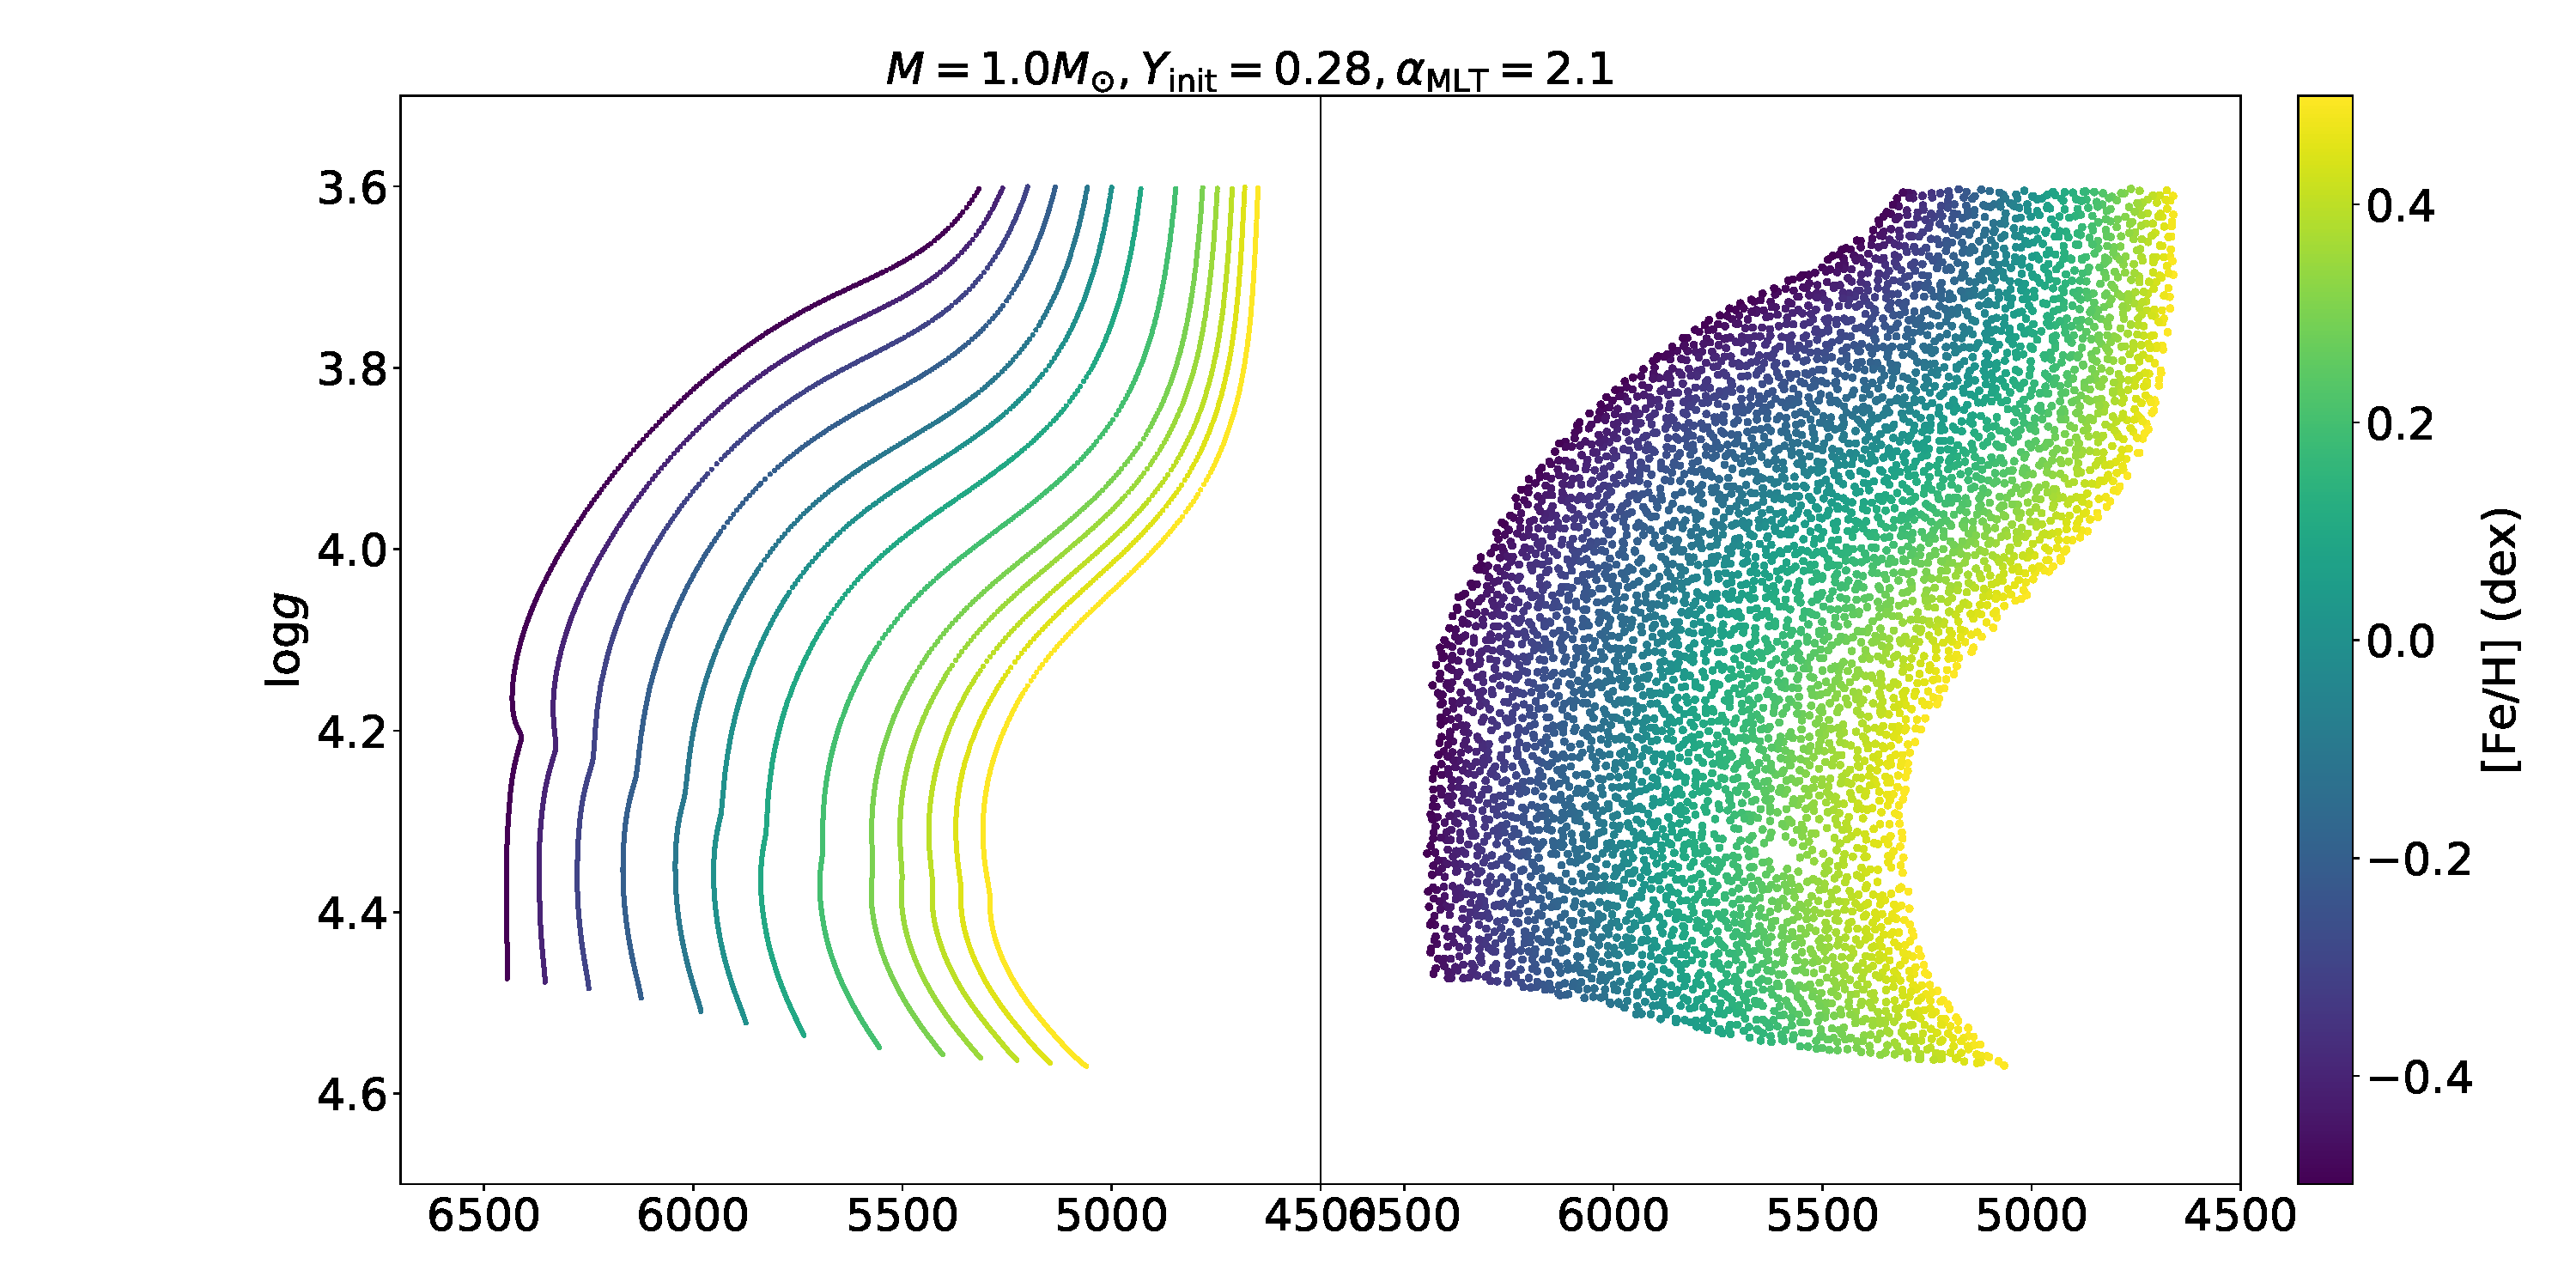
\includegraphics[width=1.2\columnwidth]{5d-au-feh.pdf}
	%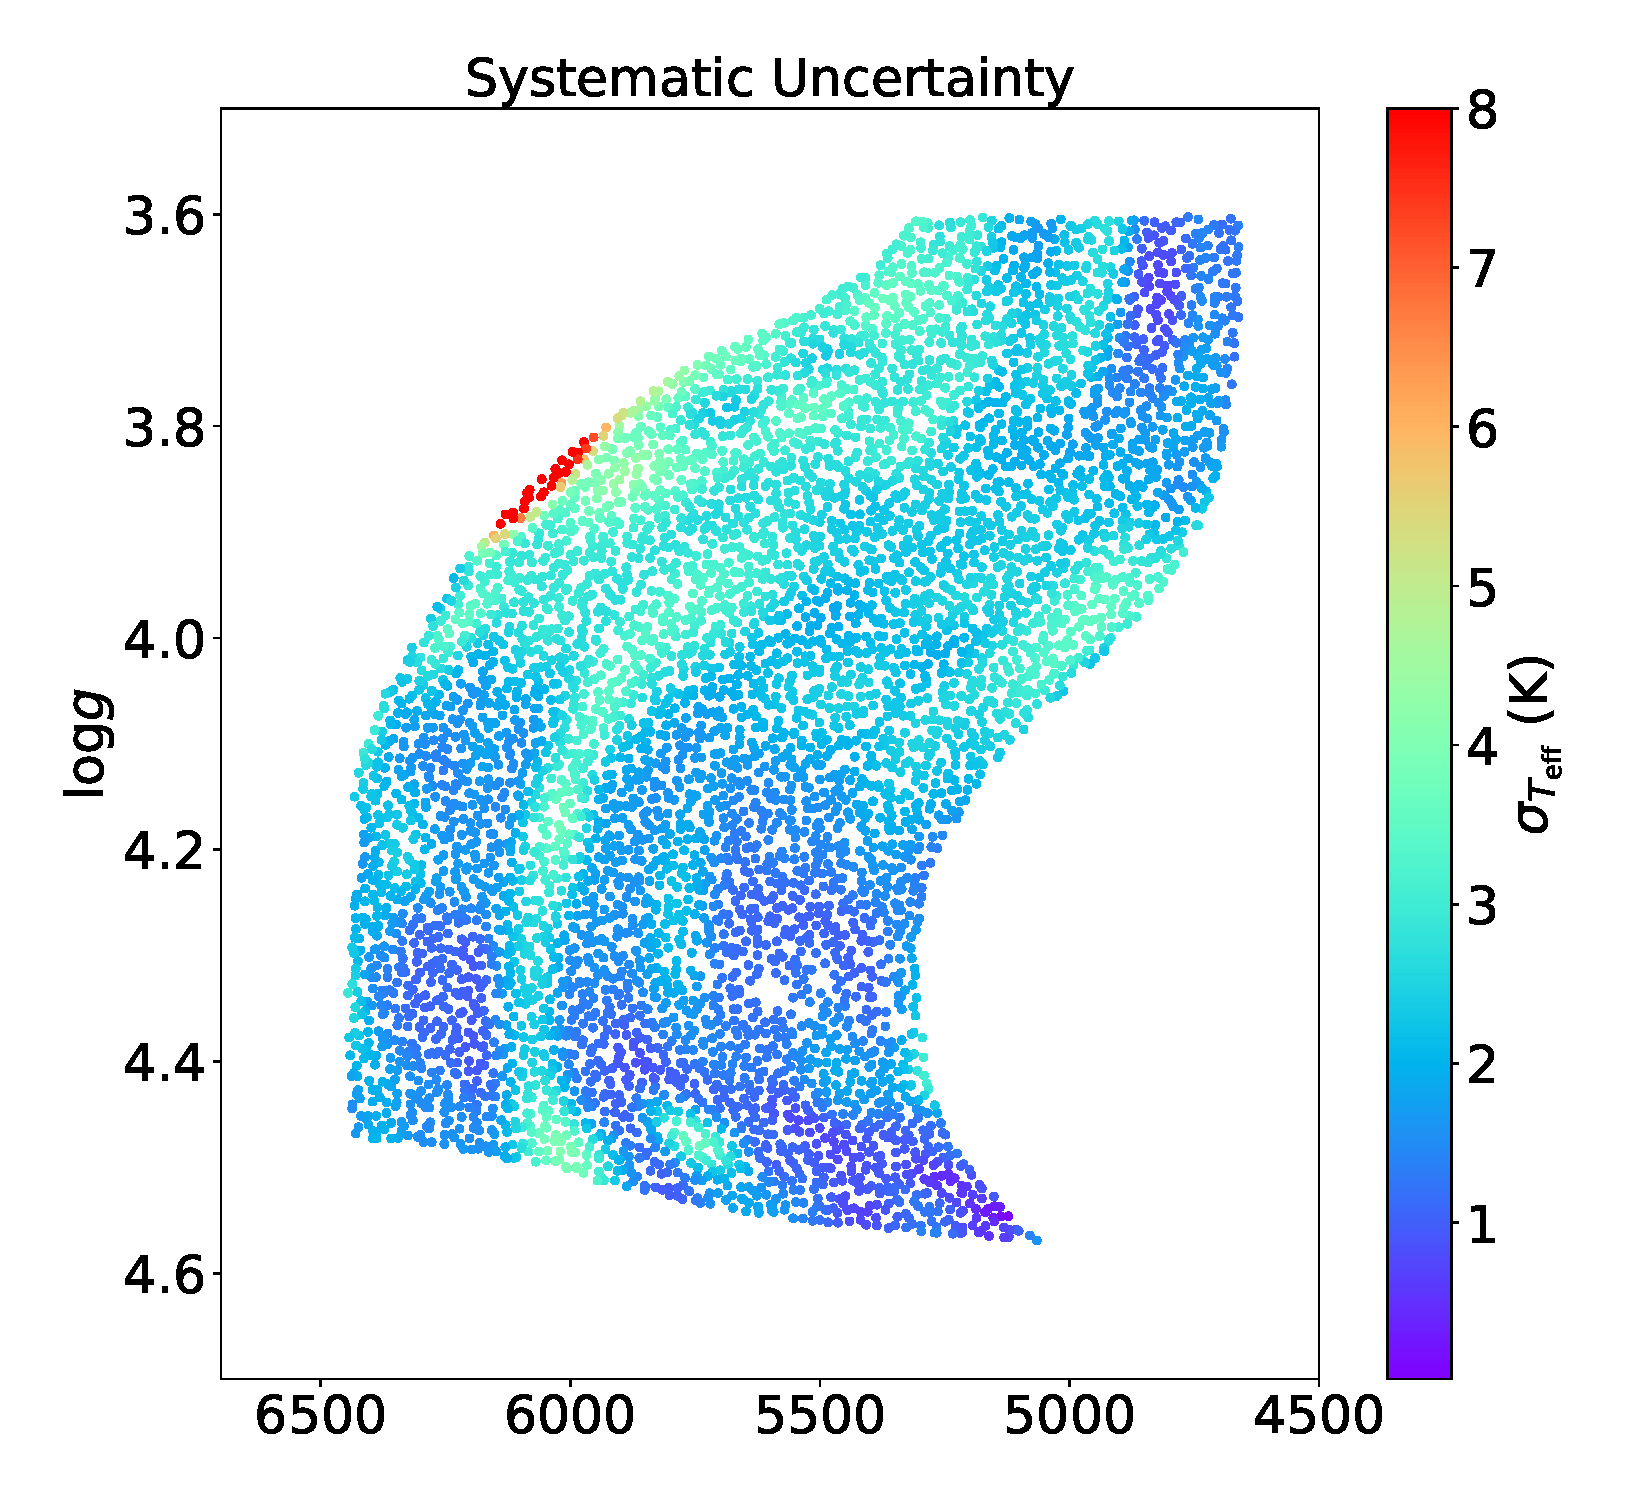
\includegraphics[width=0.65\columnwidth]{5d-au-feh-sys.pdf}
	%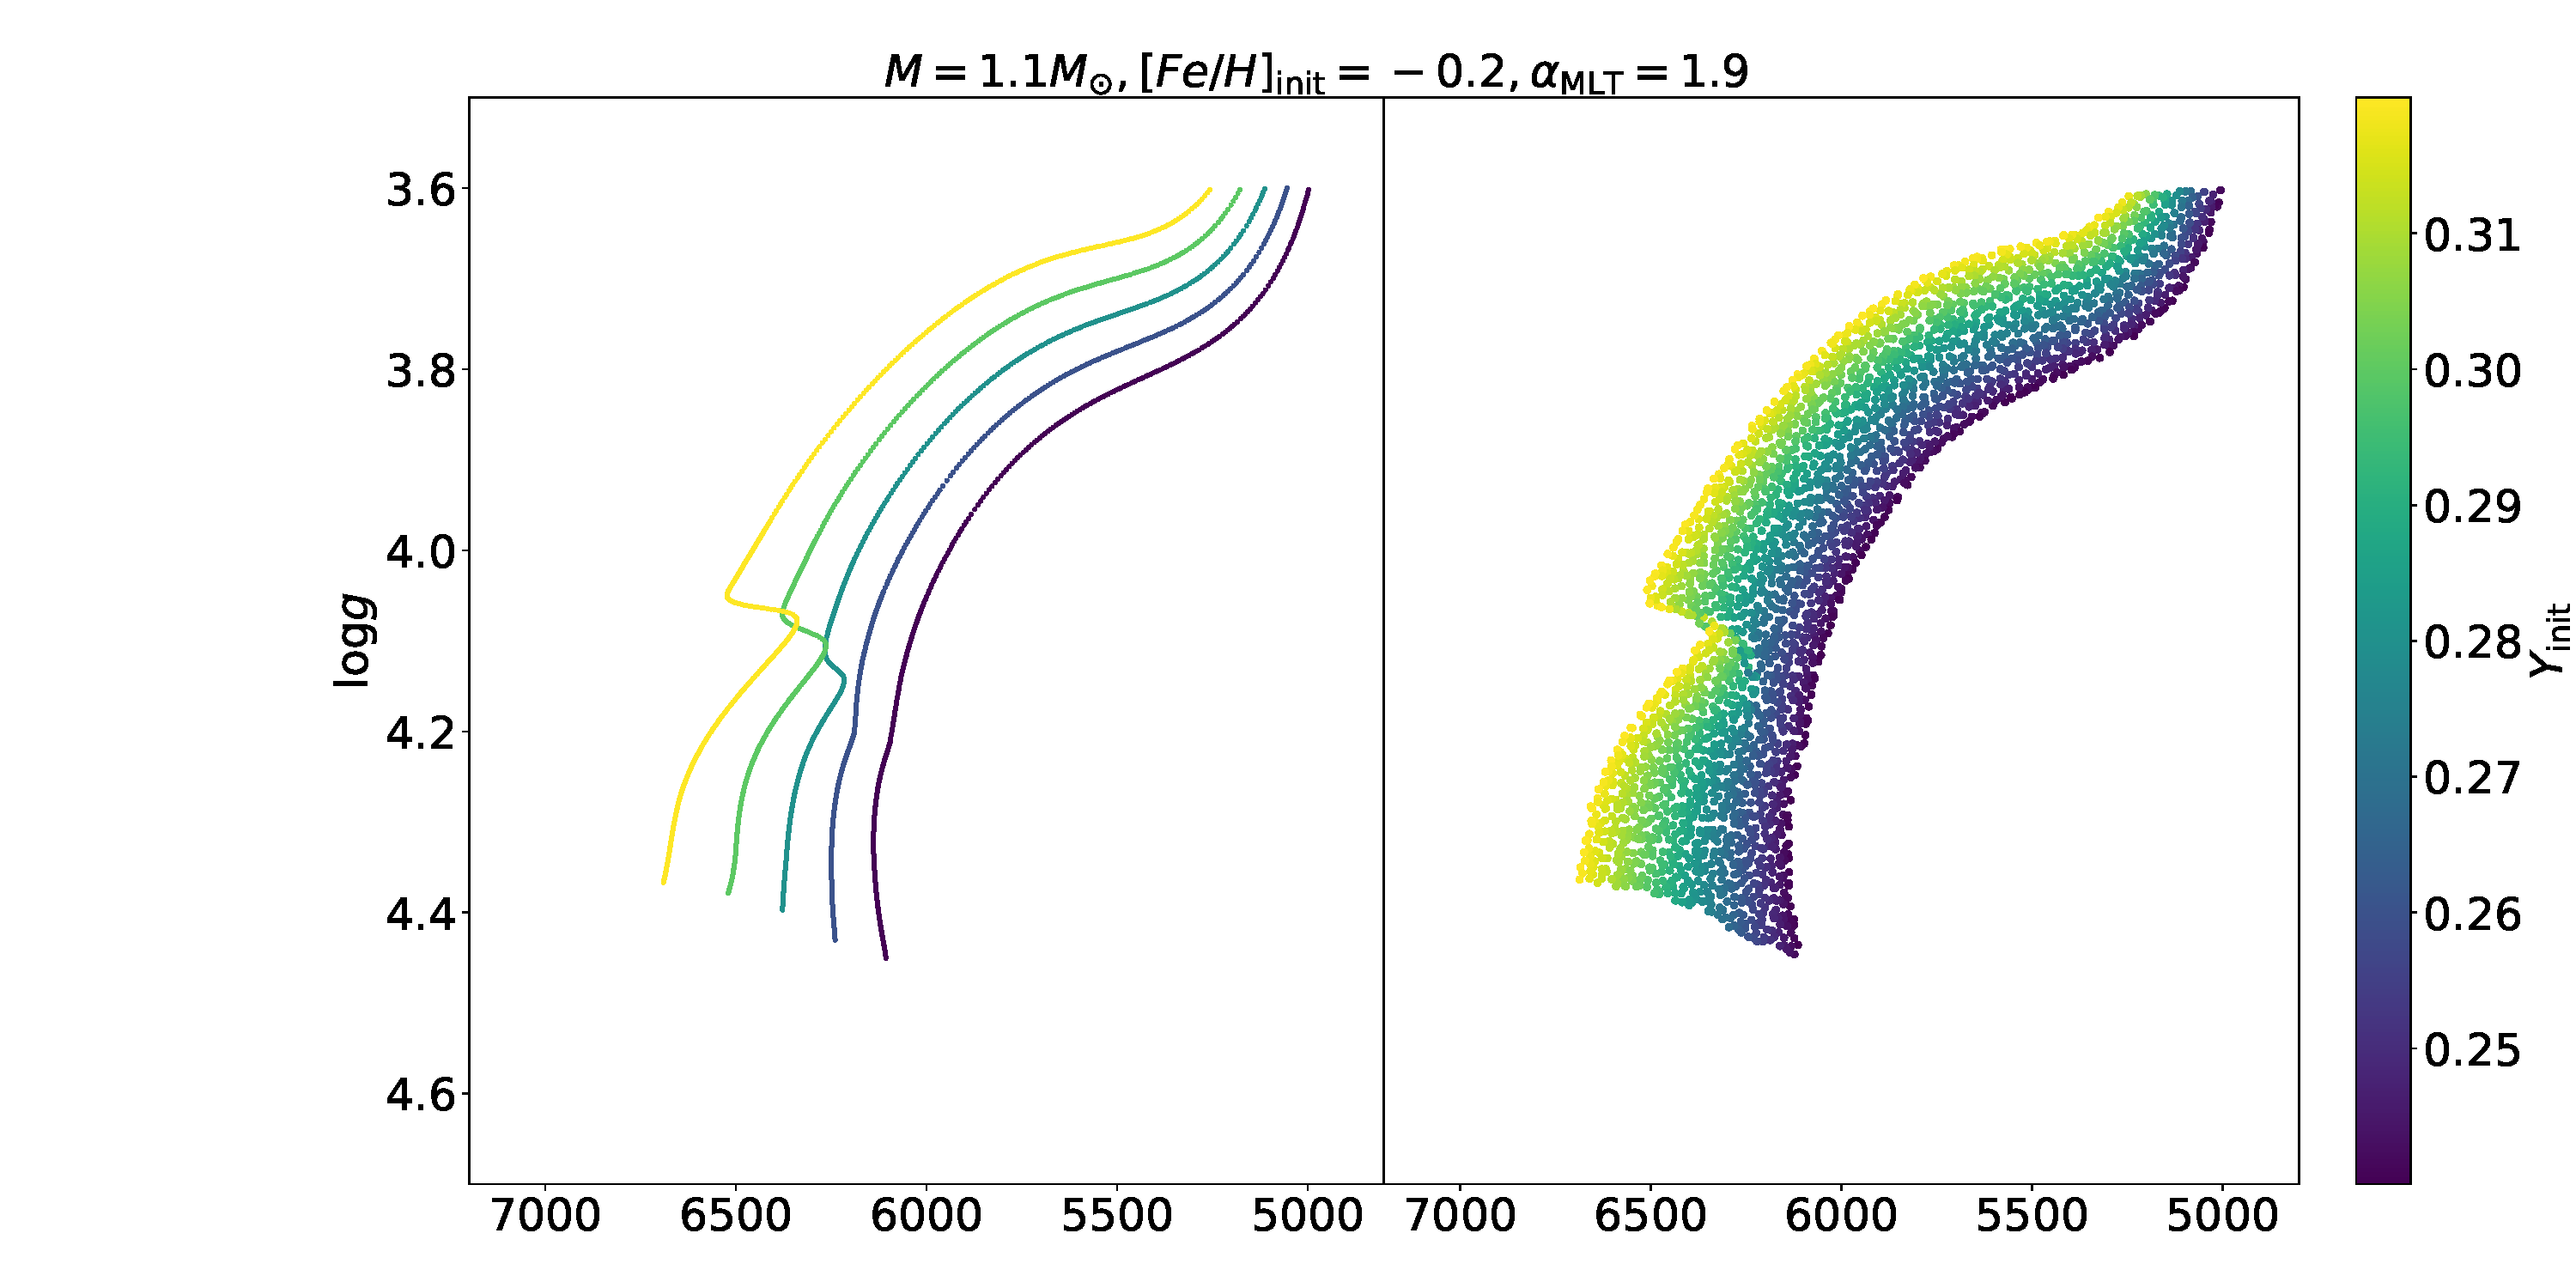
\includegraphics[width=1.2\columnwidth]{5d-au-y.pdf}
	%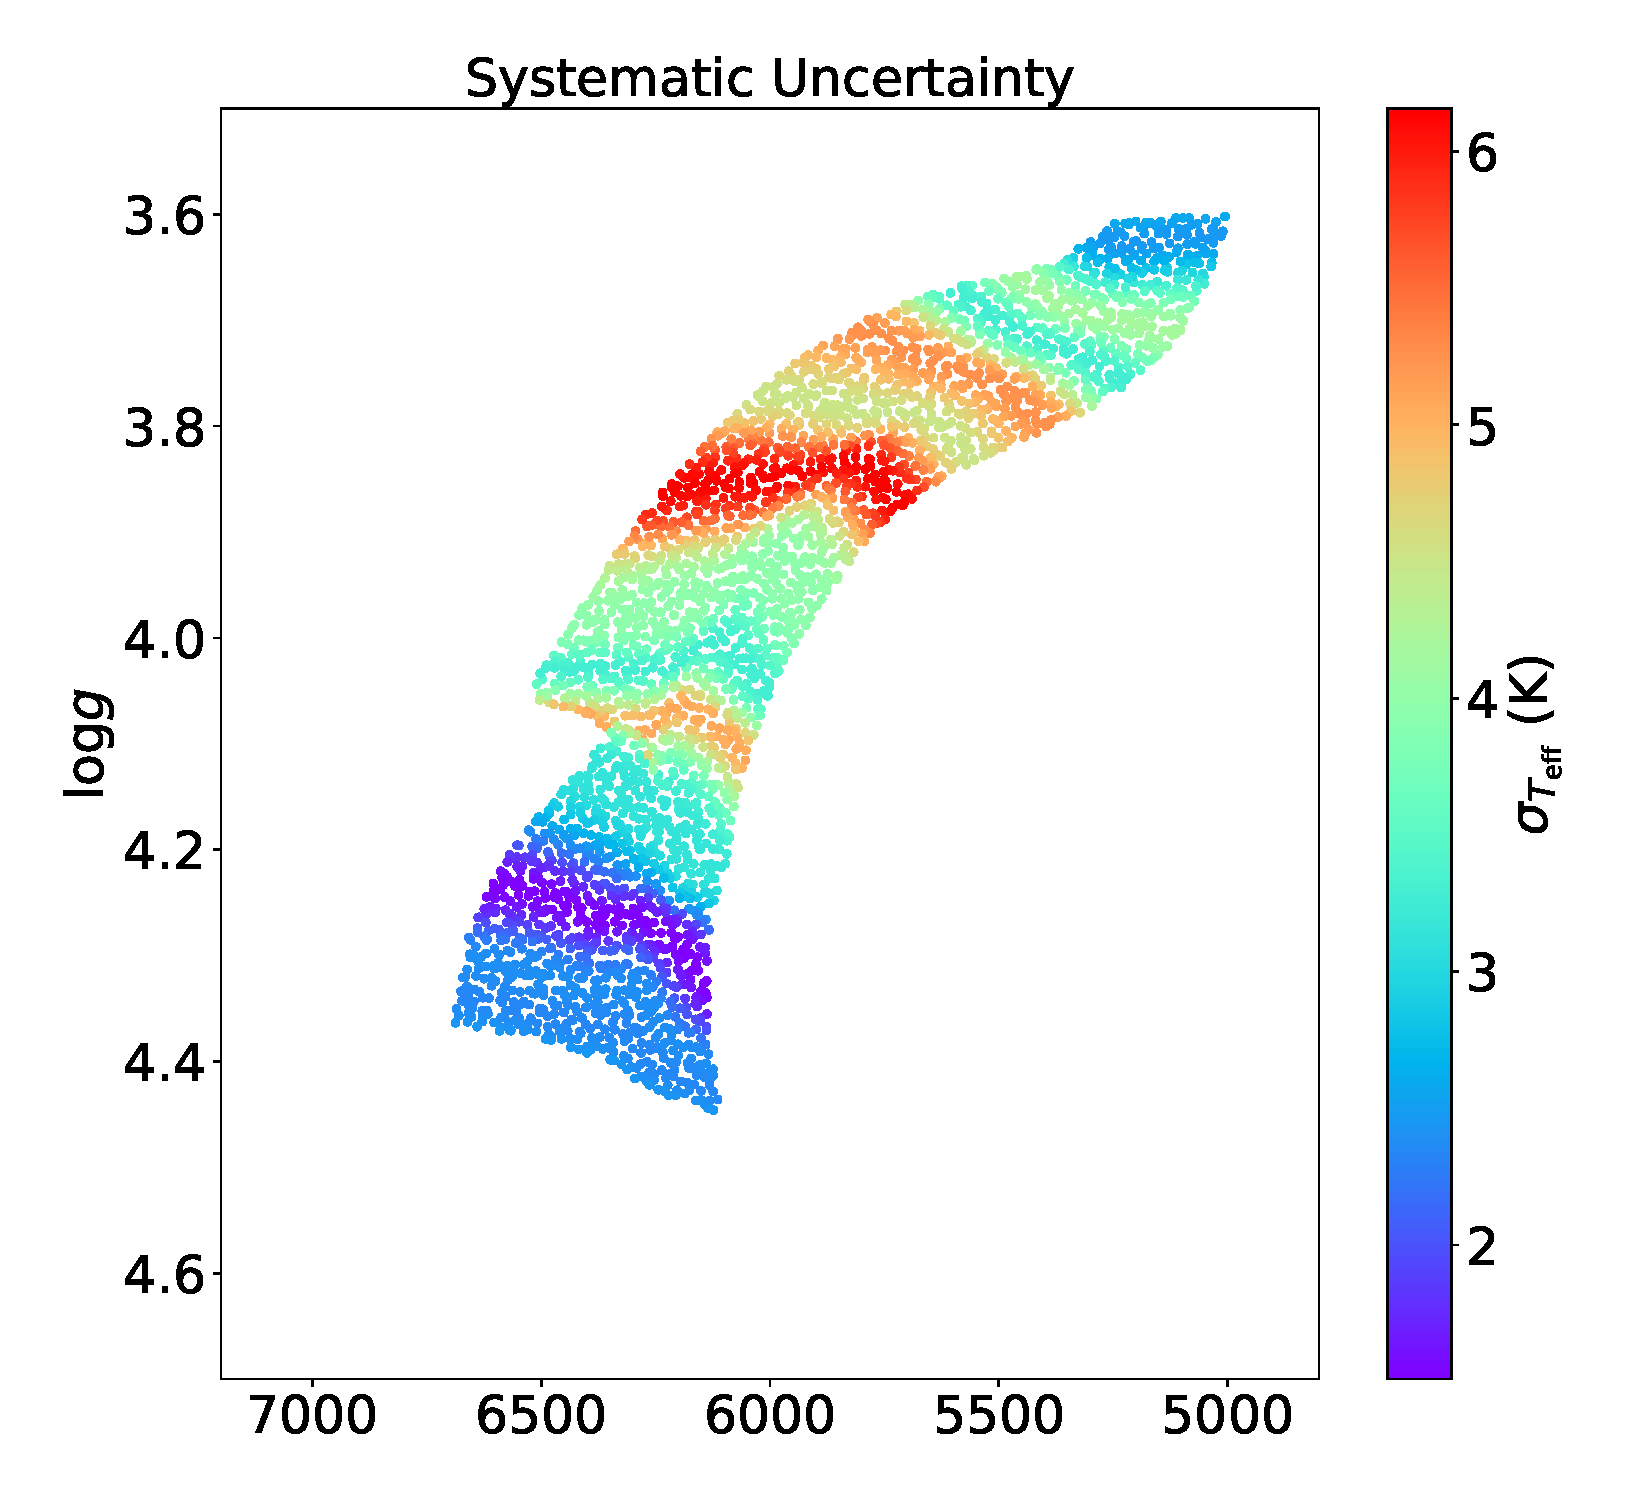
\includegraphics[width=0.65\columnwidth]{5d-au-y-sys.pdf}
	%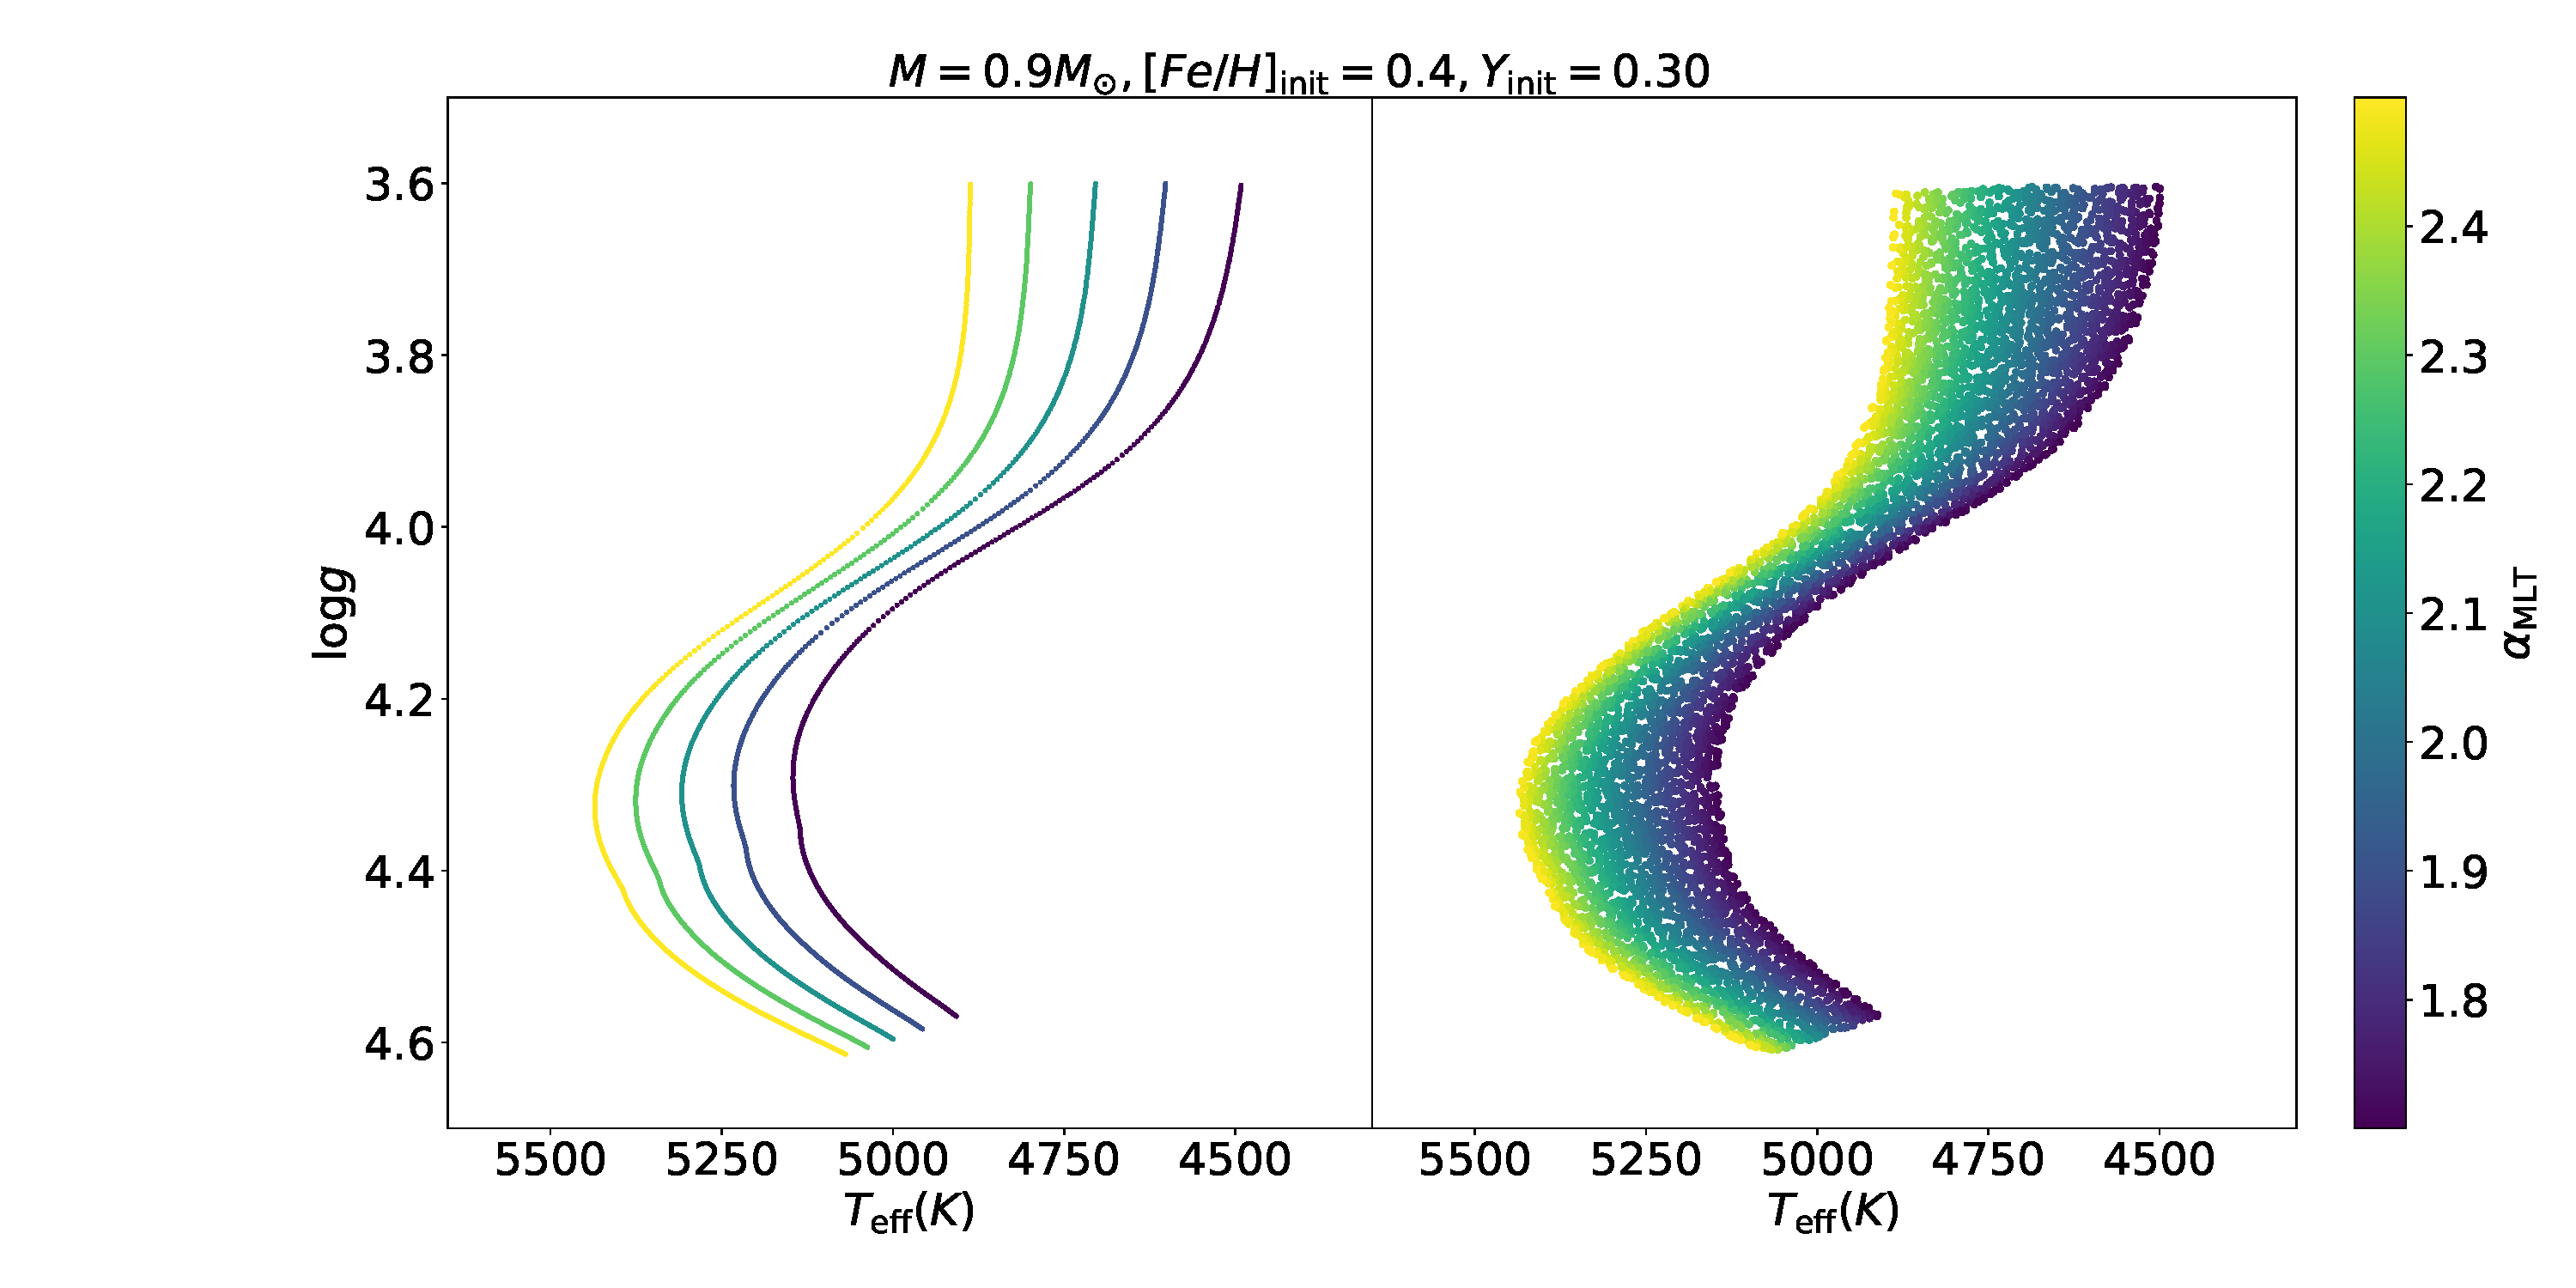
\includegraphics[width=1.2\columnwidth]{5d-au-alpha.pdf}
	%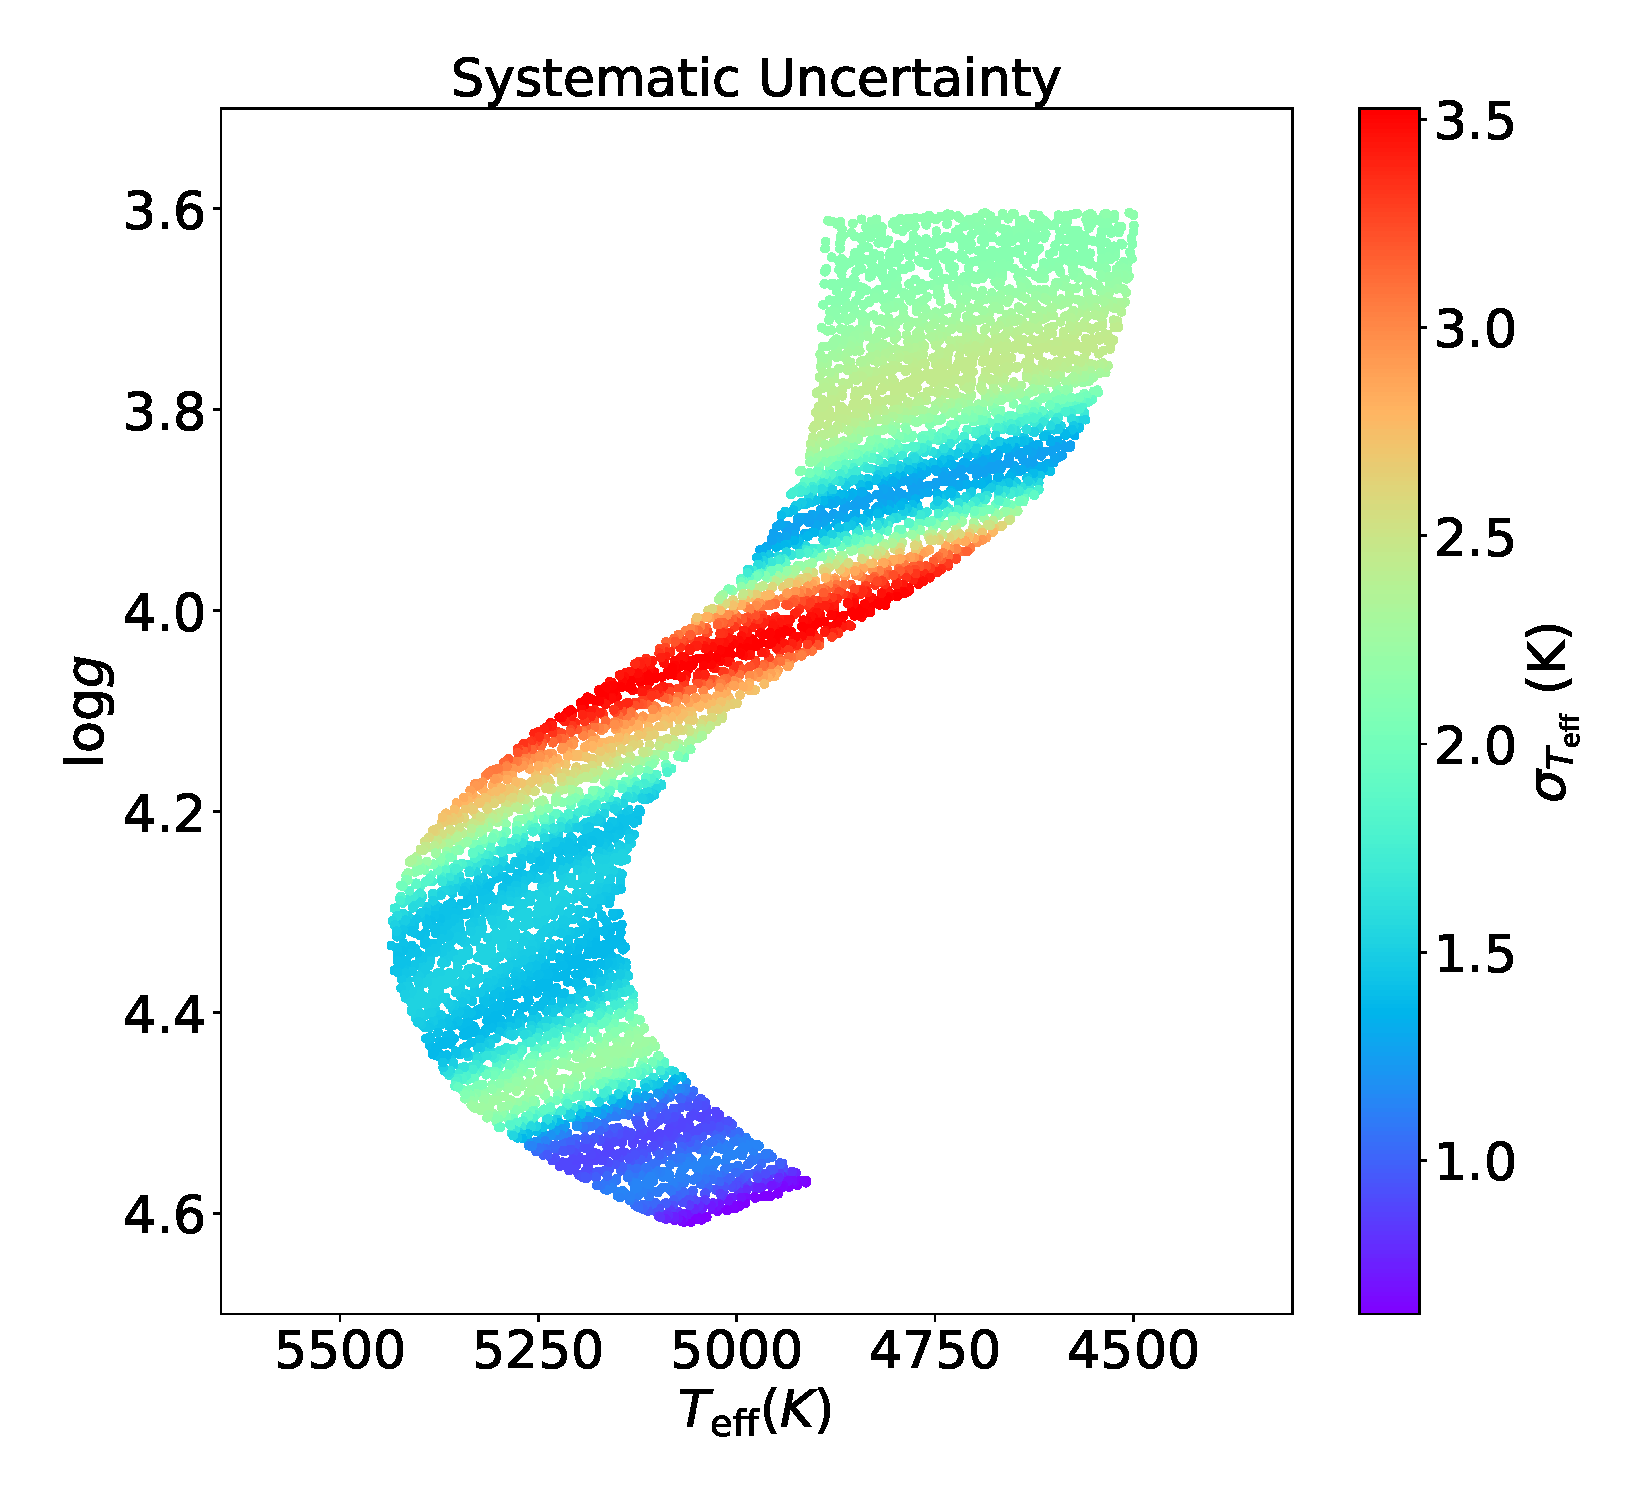
\includegraphics[width=0.65\columnwidth]{5d-au-alpha-sys.pdf}
    \caption{ Left: a GP-trained Kiel diagram compared with the stellar grid. Right: GP-predicted systematical uncertainties for all GP-trained models.} 
  \label{fig:5d_augmentation}
\end{figure*}

\subsection{Modelling fake stars with GP-trained models}

With the GP-trained model set, we model 100 fake stars to examine the accuracy of our method. Fake stars are randomly selected from the off-grid models. We use four observables, i.e., $T_{\rm eff}$, $\log g$, $R$, and [Fe/H]$_{\rm surf}$, as constraints. We apply typical observed uncertainty that is $\pm$50K for $T_{\rm eff}$ (high-resolution spectroscopy), $\pm0.005$dex for $\log g$ (seismology), $3\%$ for $R$ (seismology), and $\pm0.05$dex for [Fe/H]$_{\rm surf}$ (high-resolution spectroscopy). 
%
To avoid edge effect, fakes stars are selected in the range of $T_{\rm eff}$ = [4700K, 6800K], $\log g$ = [3.7, 4.6], [Fe/H]$_{\rm surf}$ = [-0.35,0.35], $M$ = [0.85,1.15], $EEP$ = [0.05,0.95], $Y_{\rm init}$ = [0.25,0.31], and $\alpha_{\rm MLT}$ = [1.8,2.4].  

We fit fake stars using the Maximum Likelihood Estimate (MLE) method. Note that the error term in MLE formula contents observed and systematic uncertainties given by GP-SYS models ($\sigma^{2} = \sigma_{obs}^{2} +  \sigma_{sys}^{2} $).
%
We present likelihood distributions of inferred stellar parameters for a representative fake star in Figure \ref{fig:fit_comparison}. The results based on grid modelling are also plotted as comparisons. 
%
Observed constraints for this fake star are $T_{\rm eff}$ = 4926$\pm$50K, $\log g$ = 4.536$\pm$0.005, [Fe/H]$_{\rm surf}$ =  0.34$\pm$0.05, and $R$ =  0.829$\pm$0.025$R_{\odot}$. True values of fundamental stellar parameters are $M$ = 0.861 $\rm M_{\odot}$, $\tau$ = 10.8 Gyr, $\rm [Fe/H]_{init}$ = 0.403, $Y_{\rm init}$ = 0.281, and $\alpha_{\rm MLT}$ = 2.356. 
%
Compared with the stellar grid, GP-trained model set has a completed statistical sampling and hence gives more sensible posteriors. The improvement for the age is obvious. It is under-sampled in the model grid and hence the inferred age does not actually converge. The Gird-based modelling infers an age of $7.7^{+3.2}_{-4.2}$Gyr, while GP-based modelling gives $8.3^{+2.6}_{-2.8}$Gyr. Compared with the true value (10.8 Gyr), GP determines a more accurate and precise result than the grid. For initial metallicity, initial helium fraction, and the mixing-length parameter, GP makes it possible to statistically estimate these parameters and inferred $\rm[Fe/H]_{init}$ and $Y_{\rm init}$ well agree with true values. The mixing-length parameter is not constrained because no correlated observable is given. This comparison clearly shows the advantage of GP-based modelling. It overcomes the under-sampling issue of a sparse grid and improve the accuracy and precision of estimates. 

\begin{figure*}
	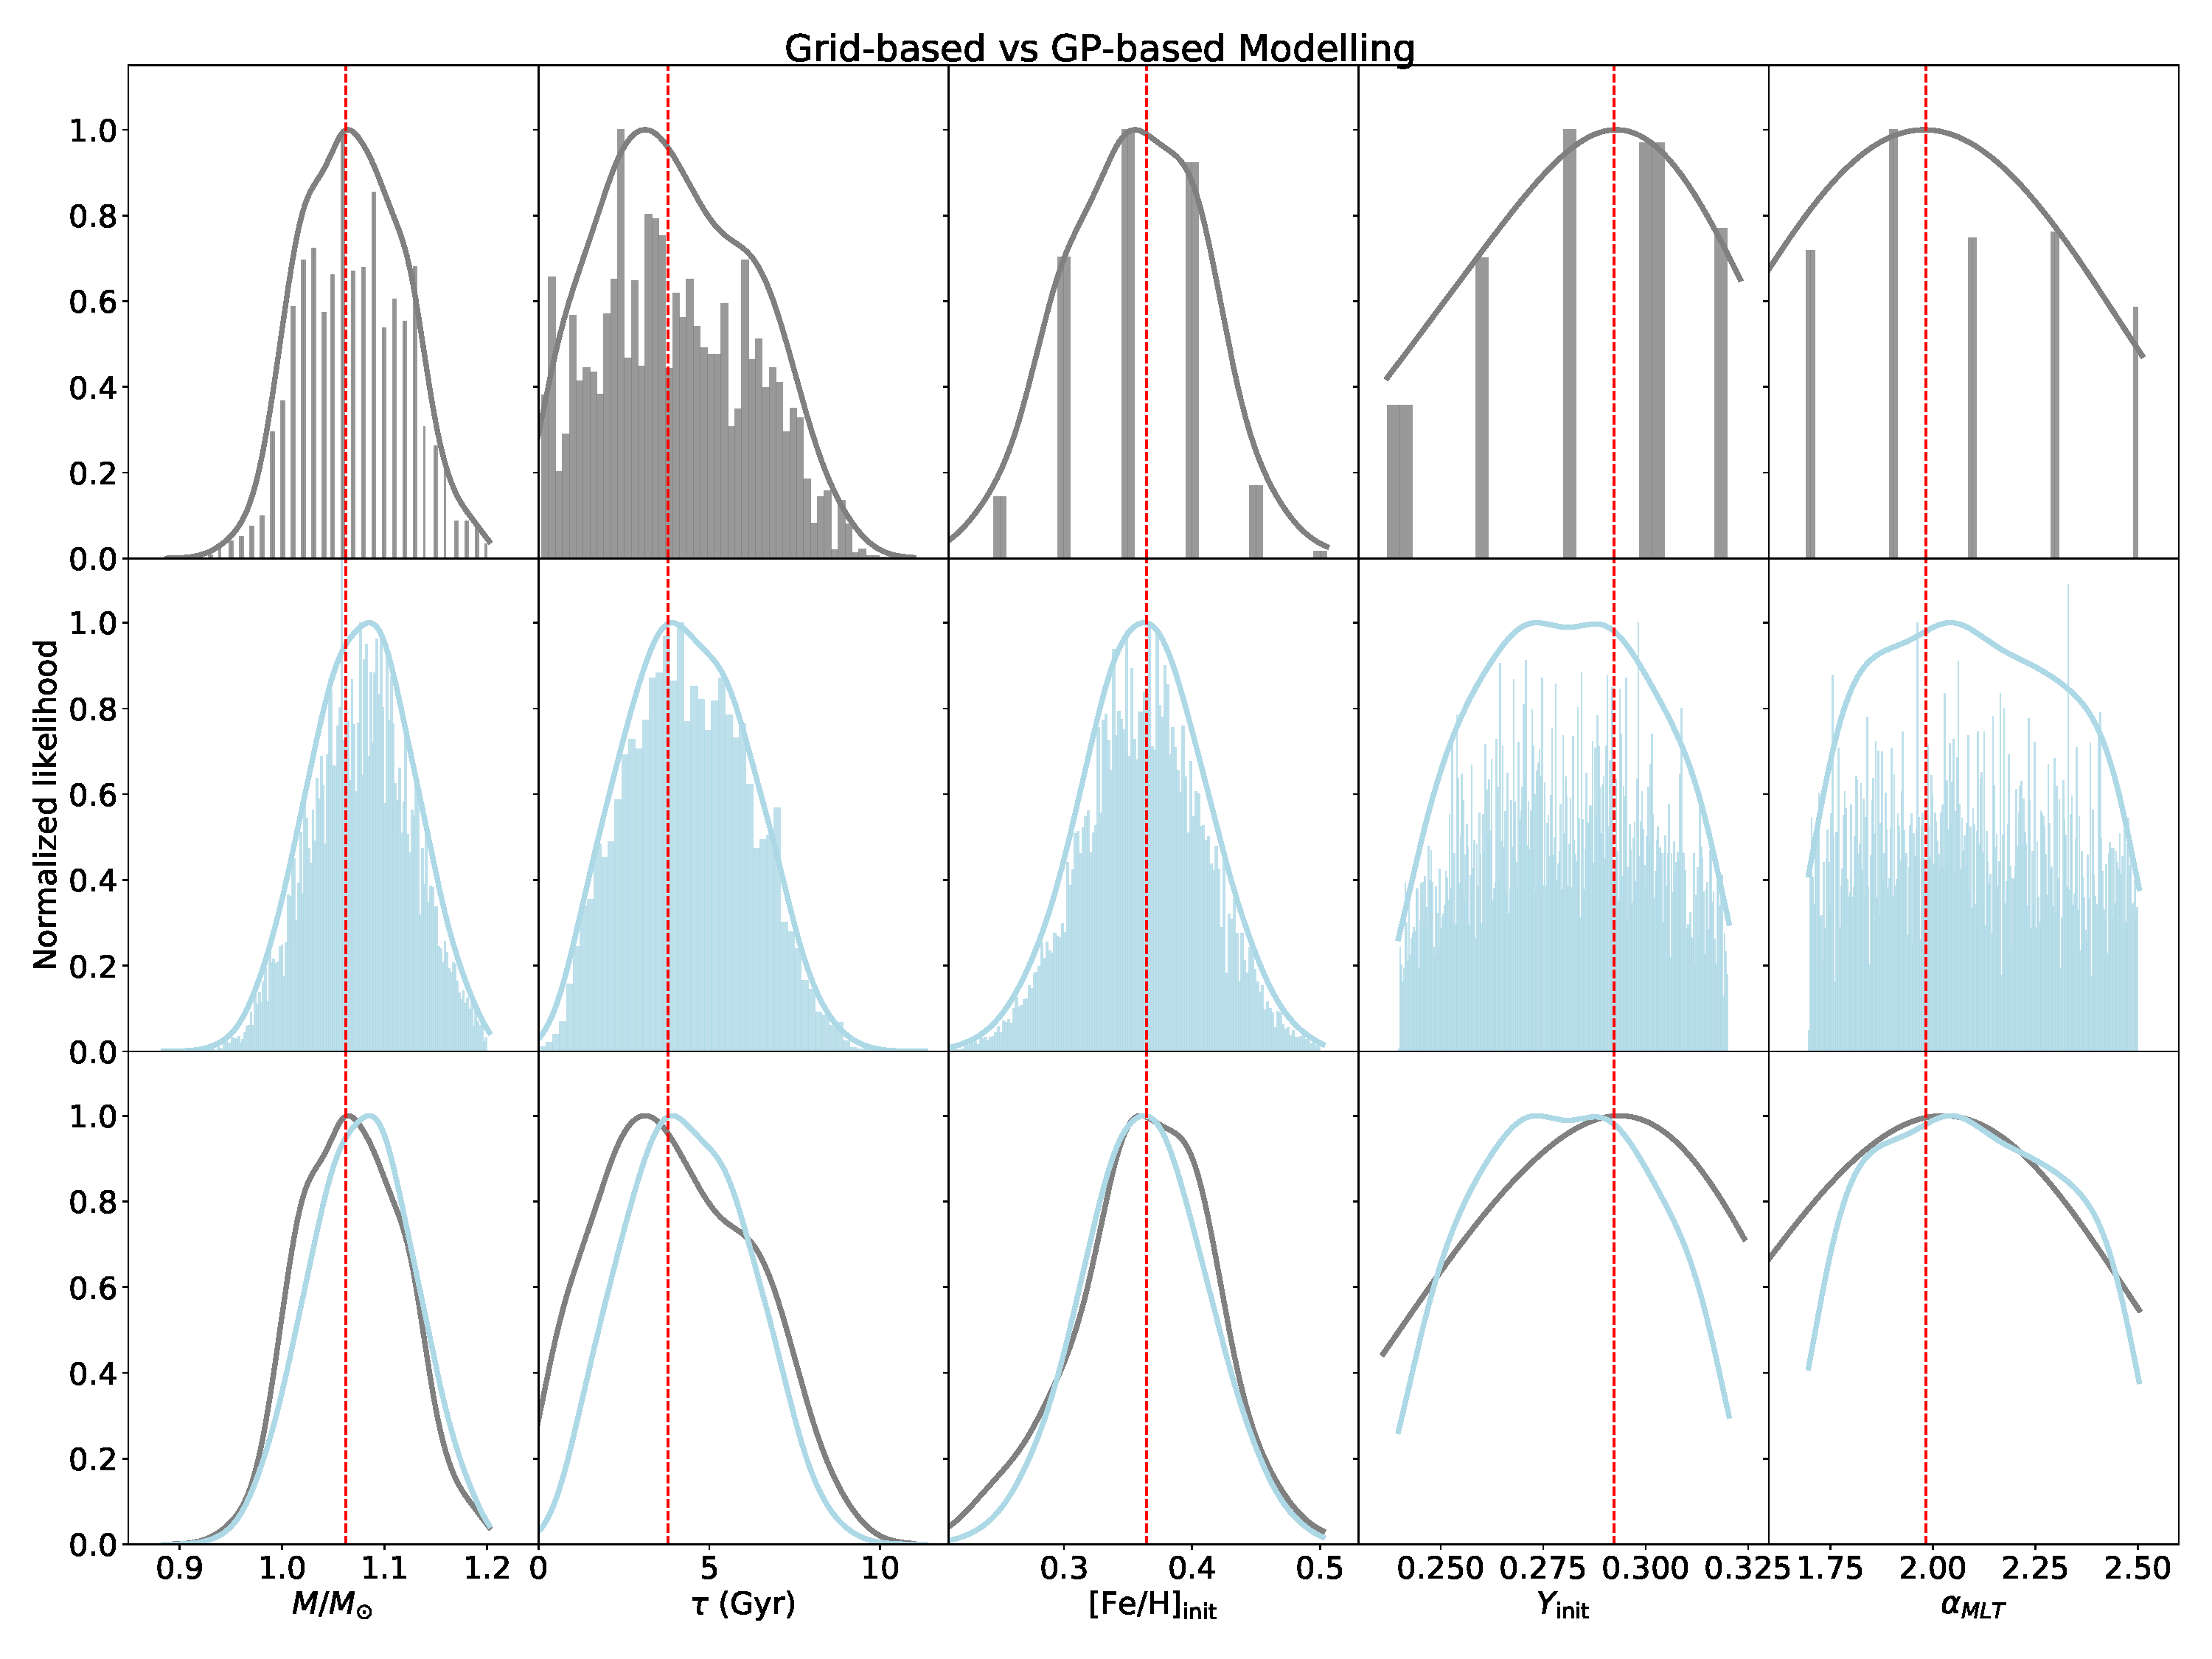
\includegraphics[width=1.9\columnwidth]{gp_fitting.pdf}
    \caption{Probability distributions of estimated fundamental parameters from grid-based (Top) and GP-based modelling (Bottom) for a fake star. Observed constraints for this fake star are $T_{\rm eff}$ = 4926$\pm$50K, $\log g$ = 4.536$\pm$0.005, [Fe/H]$_{\rm surf}$ =  0.34$\pm$0.05, and $R$ =  0.829$\pm$0.025$R_{\odot}$. True values of fundamental parameters are $M$ = 0.861 $\rm N_{\odot}$, $\tau$ = 10.8 Gyr, $\rm [Fe/H]_{init}$ = 0.403, $Y_{\rm init}$ = 0.281, $\alpha_{\rm MLT}$ = 2.356, which are represented by blue dashes.} 
  \label{fig:fit_comparison}
\end{figure*}

We now examine the accuracy of inferred mass and age of GP-based modelling. This can be done by comparing the offset (truth - estimated value) with the estimated uncertainty. If the offset is average zero and its scatter consists with typical estimated uncertainty, it would indicate that the offset is just the random error.   
%
We make marginal likelihood distributions for each fake star and measure the 16th, 50th, and 84th percentile values to estimate the mass and the age. The comparison between true and estimated values is demonstrated in Figure \ref{fig:fake_test}. Mass offsets are around zero and the scatter range (0.032$\rm M_{\odot}$) is smaller than the typical estimated uncertainty (0.04$\rm M_{\odot}$). Age differences also has a mean value at approximate zero. The scatter is relatively large compared with the case for mass but still reasonably consistent with the estimated uncertainty: offsets of 96 fake stars are within 1-$\sigma$ (1.6 Gyr) and the rest 4 stars slightly exceeds up to 1.7Gy. The results infer that this GP-based modelling gives reasonable accurate estimates when modelling real stars.  

\begin{figure*}
	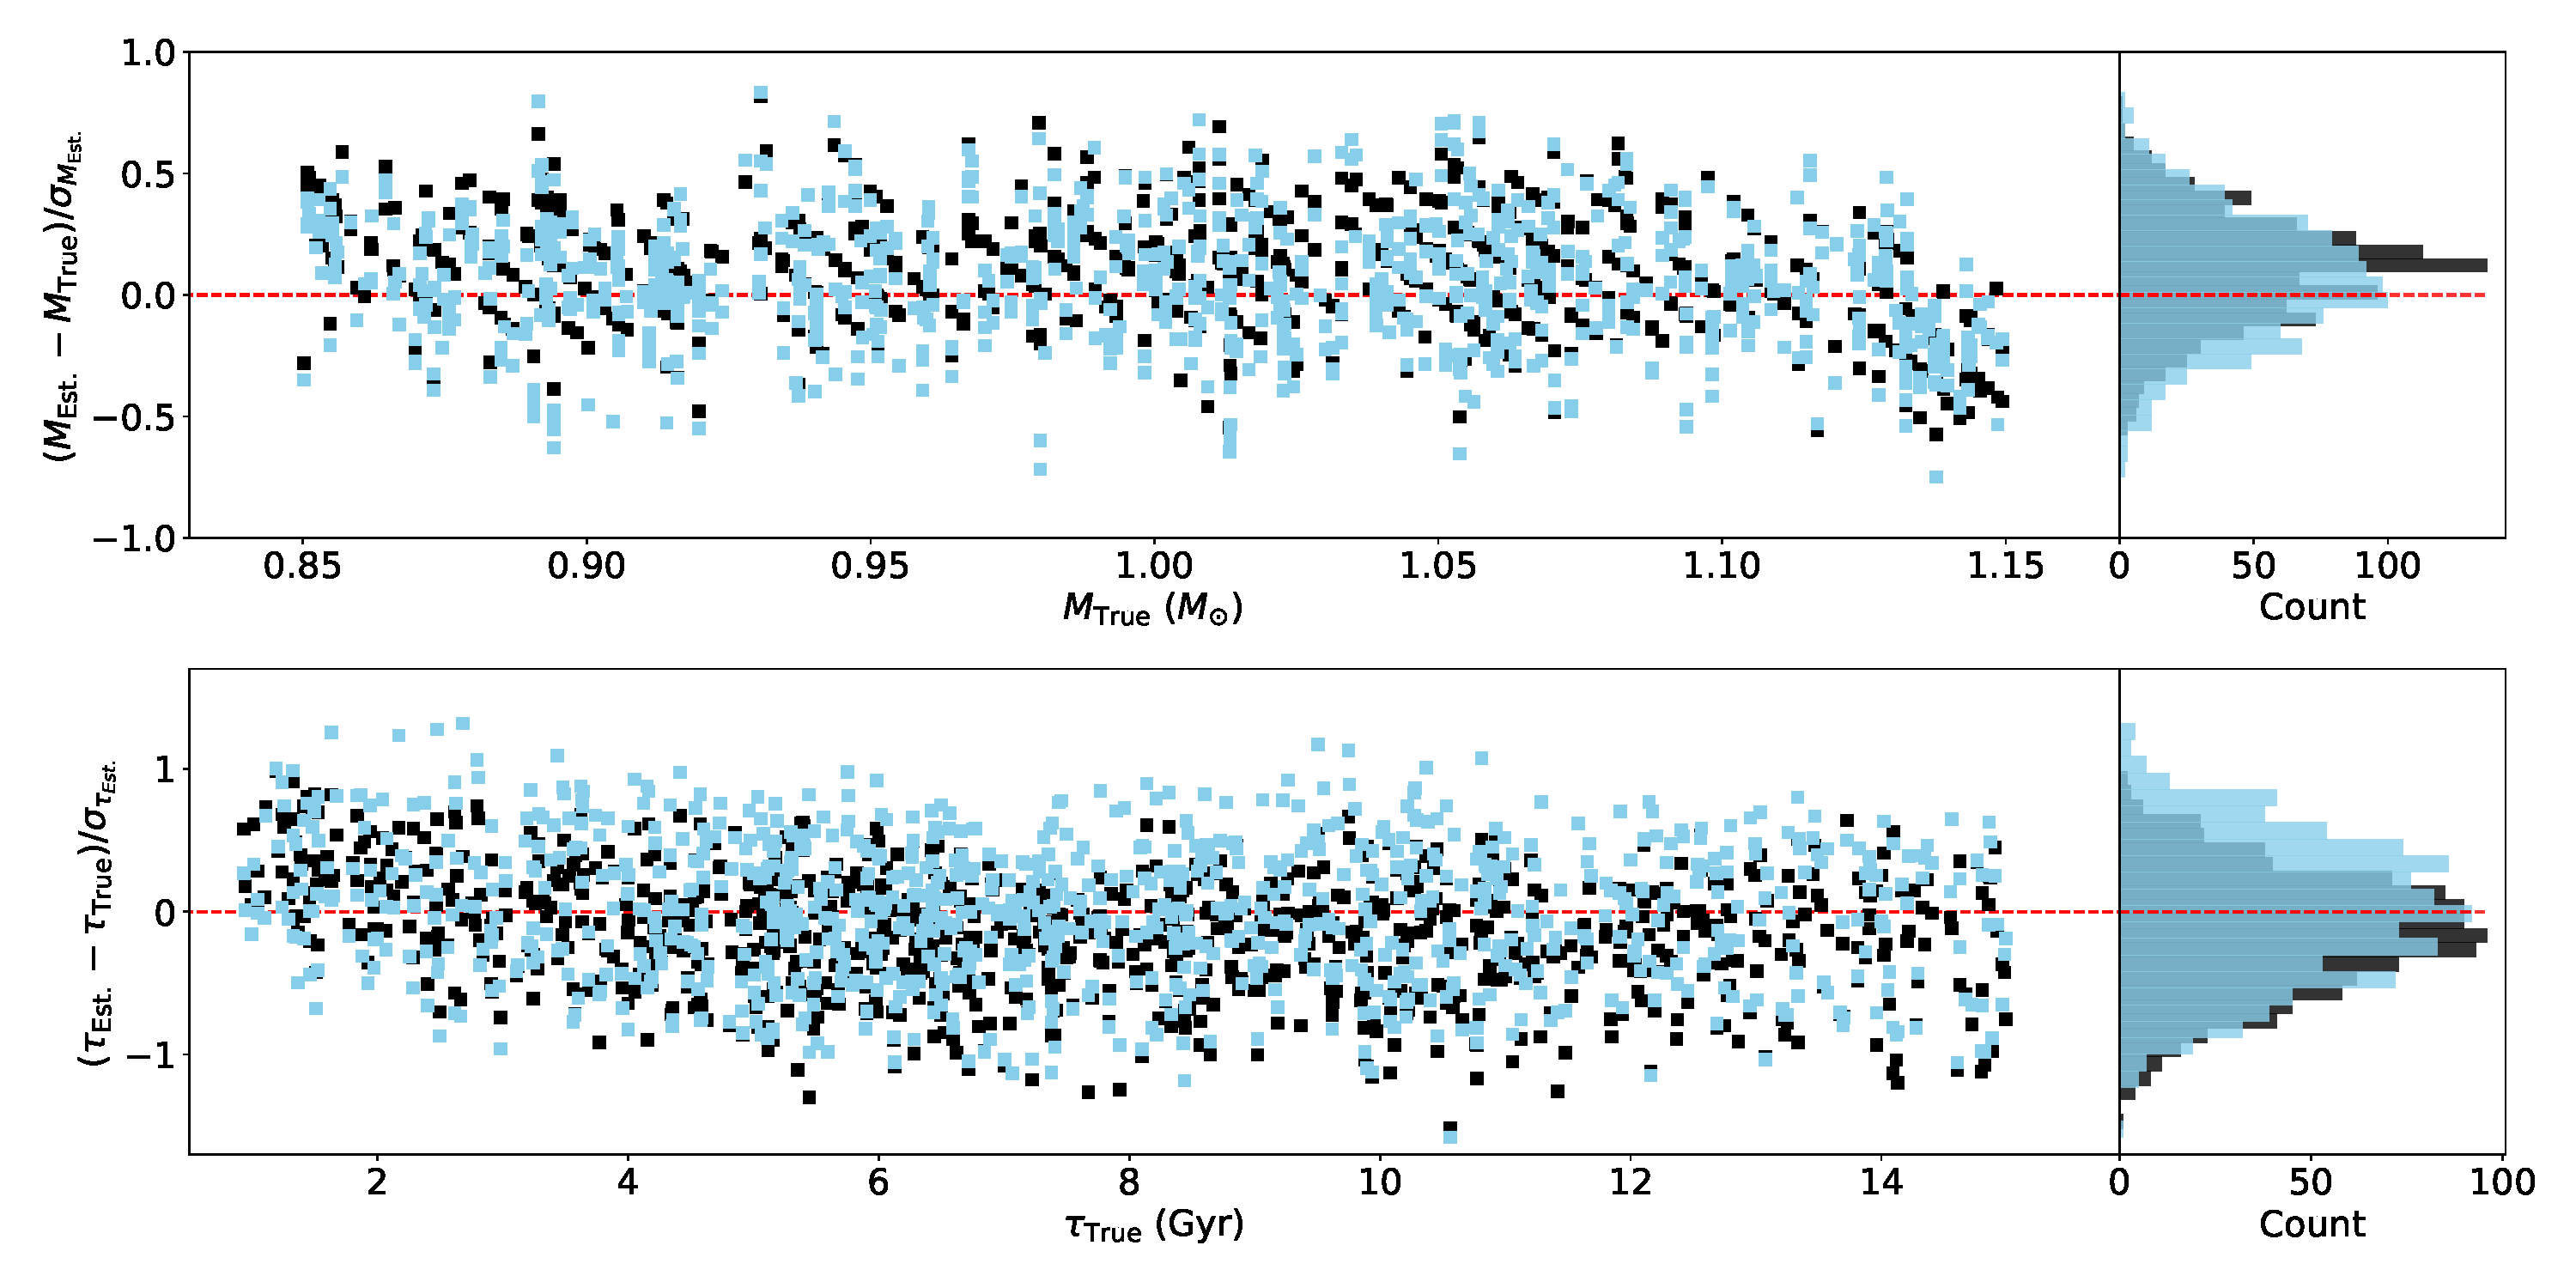
\includegraphics[width=1.8\columnwidth]{fake-stars-test.pdf}
    \caption{Differences between true and estimated masses (Top) and ages (Bottom) of 100 fake stars. Count distributions of offsets are demonstrated on the right side.} 
  \label{fig:fake_test}
\end{figure*}









